\documentclass[a4paper]{article}

\def\npart {III}
\def\nterm {Michaelmas}
\def\nyear {2016}
\def\nlecturer {R.\ Jozsa}
\def\ncourse {Quantum Computation}
\def\nofficial {https://www.qi.damtp.cam.ac.uk/node/261}

\usepackage{myheader}

\makeatletter
\DeclareRobustCommand{\rvdots}{%
  \vbox{
    \baselineskip4\p@\lineskiplimit\z@
    \kern-\p@
    \hbox{.}\hbox{.}\hbox{.}
  }
}
\newcommand\addstate[3]{
  \pgfmathsetmacro{\y@y}{-#2 * 0.7};
  \pgfmathsetmacro{\x@x}{#3};
  \node [left] at (0, \y@y) {#1};
  \draw (0, \y@y) -- (\x@x, \y@y);
}
\newcommand\addstateend[4]{
  \pgfmathsetmacro{\y@y}{-#2 * 0.7};
  \pgfmathsetmacro{\x@x}{#3};
  \node [left] at (0, \y@y) {#1};
  \node [right] at (\x@x, \y@y) {#4};
  \draw (0, \y@y) -- (\x@x, \y@y);
}

\newcommand\addoperator[3]{
  \node [draw, rectangle, fill=white] at (#3, -#2 * 0.7) {#1};
}
\newcommand\addbigoperator[5]{
  \pgfmathsetmacro{\y@s}{-#2 * 0.7 + 0.2};
  \pgfmathsetmacro{\y@t}{-#3 * 0.7 - 0.2};
  \pgfmathsetmacro{\x@s}{#4};
  \pgfmathsetmacro{\x@t}{#5};
  \pgfmathsetmacro{\x@c}{(\x@s + \x@t)/2};
  \pgfmathsetmacro{\y@c}{(\y@s + \y@t)/2};

  \draw [fill=white] (\x@s, \y@s) rectangle (\x@t, \y@t);
  \node at (\x@c, \y@c) {#1};
}

\newcommand\addMQCstate [3] {
  \pgfmathsetmacro{\x@x}{#3 * 1.5 - 1};
  \node [left] at (0, -#2) {#1};
  \draw (0, -#2) -- (\x@x, -#2);
}

\newcommand\addJ[3]{
  \pgfmathsetmacro{\x@x}{#3 * 1.5 - 0.5};
 \node [draw, rectangle, fill=morange!30!white, minimum height=0.65cm, minimum width=1cm] at (\x@x, -#2) {$\qJ(#1)$};
}
\newcommand\addX[3]{
  \pgfmathsetmacro{\x@x}{#3 * 1.5 - 0.5};
  \node [draw, rectangle, fill=mgreen!30!white, minimum height=0.65cm, minimum width=1cm] at (\x@x, -#2) {$\qX^{#1}$};
}
\newcommand\addZ[3]{
  \pgfmathsetmacro{\x@x}{#3 * 1.5 - 0.5};
  \node [draw, rectangle, fill=mblue!30!white, minimum height=0.65cm, minimum width=1cm] at (\x@x, -#2) {$\qZ^{#1}$};
}
\newcommand\addPhantom[2]{
  \pgfmathsetmacro{\x@x}{#2 * 1.5 - 0.5};
  \node [minimum height=0.65cm, minimum width=1cm] at (\x@x, -#1) {};
}
\newcommand\drawvert[3]{
  \pgfmathsetmacro{\x@x}{#3 * 1.5 - 0.5};
  \draw (\x@x, -#1) node [circ] {} -- (\x@x, -#2) node [circ] {};
}
\newcommand\measurestate[4] {
  \pgfmathsetmacro{\y@y}{-#3 - 0.05};
  \pgfmathsetmacro{\x@x}{#4 + 0.05};
  \draw [-latex'] (\x@x, \y@y) -- +(0.4, -0.4) node [right] {#2};
  \node [above] at (#4, -#3) {#1};
}

\newcommand{\qCX}{\mathsf{CX}}
\newcommand{\qCZ}{\mathsf{CZ}}
\newcommand{\qE}{\mathsf{E}}
\newcommand{\qJ}{\mathsf{J}}
\newcommand{\qM}{\mathsf{M}}
\newcommand{\qQFT}{\mathsf{QFT}}
\newcommand{\qH}{\mathsf{H}}
\newcommand{\qP}{\mathsf{P}}
\newcommand{\qT}{\mathsf{T}}
\newcommand{\qX}{\mathsf{X}}
\newcommand{\qY}{\mathsf{Y}}
\newcommand{\qZ}{\mathsf{Z}}
\newcommand{\qcd}{\mathsf{c}\operatorname{-}}
\newcommand{\AND}{\mathsf{AND}}
\newcommand{\NOT}{\mathsf{NOT}}
\newcommand{\OR}{\mathsf{OR}}

\makeatother

\begin{document}
\maketitle
{\small
\setlength{\parindent}{0em}
\setlength{\parskip}{1em}

Quantum mechanical processes can be exploited to provide new modes of information processing that are beyond the capabilities of any classical computer. This leads to remarkable new kinds of algorithms (so-called quantum algorithms) that can offer a dramatically increased efficiency for the execution of some computational tasks. Notable examples include integer factorisation (and consequent efficient breaking of commonly used public key crypto systems) and database searching. In addition to such potential practical benefits, the study of quantum computation has great theoretical interest, combining concepts from computational complexity theory and quantum physics to provide striking fundamental insights into the nature of both disciplines.

The course will cover the following topics:

Notion of qubits, quantum logic gates, circuit model of quantum computation. Basic notions of quantum computational complexity, oracles, query complexity.

The quantum Fourier transform. Exposition of fundamental quantum algorithms including the Deutsch-Jozsa algorithm, Shor's factoring algorithm, Grovers searching algorithm.

A selection from the following further topics (and possibly others):
\begin{enumerate}
  \item Quantum teleportation and the measurement-based model of quantum computation;
  \item Lower bounds on quantum query complexity;
  \item Phase estimation and applications in quantum algorithms;
  \item Quantum simulation for local hamiltonians.
\end{enumerate}

\subsubsection*{Pre-requisites}
It is desirable to have familiarity with the basic formalism of quantum mechanics especially in the simple context of finite dimensional state spaces (state vectors, Dirac notation, composite systems, unitary matrices, Born rule for quantum measurements). Prerequisite notes will be provided on the course webpage giving an account of the necessary material including exercises on the use of notations and relevant calculational techniques of linear algebra. It would be desirable for you to look through this material at (or slightly before) the start of the course. Any encounter with basic ideas of classical theoretical computer science (complexity theory) would be helpful but is not essential.
}
\tableofcontents

\setcounter{section}{-1}
\section{Introduction}
Quantum computation is currently a highly significant and important subject, and is very active in international research.

First of all, it is a fundamental connection between physics and computing. We can think of physics as computing, where in physics, we label states with parameters (i.e.\ numbers), and physical evolution changes these parameters. So we can think of these parameters as encoding information, and physical evolution changes the information. Thus, this evolution can be thought of as a computational process.

More strikingly, we can also view computing as physics! We all have computers, and usually represent information as bits, 0 or 1. We often think of computation as manipulation of these bits, i.e.\ as discrete maths. However, there is no actual discrete bits --- when we build a computer, we need physical devices to represent these bits. When we run a computation on a computer, it has to obey the laws of physics. So we arrive at the idea that the limits of computation are not a part of mathematics, but depend on the laws of physics. Thus, we can associate a ``computing power'' with any theory of physics!

On the other hand, there is also a technology/engineering aspect of quantum computation. Historically, we have been trying to reduce the size of computers. Eventually, we will want to try to achieve miniaturization of computer components to essentially the subatomic scale. The usual boolean operations we base our computations on do not work so well on this small scale, since quantum effects start to kick in. We could try to mitigate these quantum issues and somehow force the bits to act classically, but we can also embrace the quantum effects, and build a quantum computer! There is a lot of recent progress in quantum technology. We are now expecting a 50-qubit quantum computer in full coherent control soon. However, we are not going to talk about implementation in this course.

Finally, apart from the practical problem of building quantum computers, we also have theoretical quantum computer science, where we try to understand how quantum algorithms behave. This is about how we can actually exploit quantum physical facts for computational possibilities beyond classical computers. This will be the focus of the course.

\section{Classical computation theory}
To appreciate the difference between quantum and classical computing, we need to first understand classical computing. We will only briefly go over the main ideas instead of working out every single technical detail. Hence some of the definitions might be slightly vague.

We start with the notion of ``computable''. To define computability, one has to come up with a sensible mathematical model of a computer, and then ``computable'' means that theoretical computer can compute it. So far, any two sensible mathematical models of computations we manage to come up with are equivalent, so we can just pick any one of them. Consequently, we will not spend much time working out a technical definition of computable.

\begin{eg}
  Let $N$ be an integer. We want to figure out if $N$ a prime. This is clearly computable, since we can try all numbers less than $N$ and see if it divides $N$.
\end{eg}

This is not too surprising, but it turns out there are some problems that are not computable! Most famously, we have the Halting problem.
\begin{eg}[Halting problem]\index{Halting problem}
  Given the code of a computer program, we want to figure out if the computer will eventually halt. In 1936, Turing proved that this problem is uncomputable! So we cannot have a program that determines if an arbitrary program halts.
\end{eg}

For a less arbitrary problem, we have
\begin{eg}
  Given a polynomial with integer coefficients with many variables, e.g.\ $2x^2 y - 17 zw^{19} + x^5 w^3 + 1$, does this have a root in the integers? It was shown in 1976 that this problem is uncomputable as well!
\end{eg}

These results are all for classical computing. If we expect quantum computing to be somehow different, can we get around this problems? This turns out not to be the case, for the very reason that all the laws of quantum physics (e.g.\ state descriptions, evolution equations) are all computable on a classical computer (in principle). So it follows that quantum computing, being a quantum process, cannot compute any classical uncomputable problem.

Despite this limitation, quantum computation is still interesting! In practice, we do not only care about computability. We care about how efficient we are at doing the computation. This is the problem of complexity --- the complexity of a quantum computation might be much simpler than the classical counterpart.

To make sense of complexity, we need to make our notion of computations a bit more precise.

\begin{defi}[Input string]\index{input string}
  An \emph{input bit string} is a sequence of bits $x = i_1i_2 \cdots i_n$, where each $i_k$ is either $0$ or $1$. We write $B_n$ for the set of all $n$-bit string, and $B = \bigcup_{n \in \N} B_n$. The \emph{input size} is the length $n$. So in particular, if the input is regarded as an actual number, the size is not the number itself, but its logarithm.
\end{defi}

\begin{defi}[Language]
  A \term{language} is a subset $L\subseteq B$.
\end{defi}

\begin{defi}[Decision problem]
  Given a language $L$, the \term{decision problem} is to determine whether an arbitrary $x \in B$ is a member of $L$. The output is thus 1 bit of information, namely yes or no.
\end{defi}
Of course, we can have a more general task with multiple outputs, but for simplicity, we will not consider that case here.

\begin{eg}
  If $L$ is the set of all prime numbers, then the corresponding decision problem is determining whether a number is prime.
\end{eg}

We also have to talk about models of computations. We will only give an intuitive and classical description of it.
\begin{defi}[Computational model]
  A \term{computational model} is a process with discrete steps (elementary computational steps), where each step requires a constant amount of effort/resources to implement.
\end{defi}
If we think about actual computers that works with bits, we can imagine a step as an operation such as ``and'' or ``or''. Note that addition and multiplication are \emph{not} considered a single step --- as the number gets larger, it takes more effort to add or multiply them.

Sometimes it is helpful to allow some randomness.
\begin{defi}[Randomized/probabilistic computation]
  This is the same as a usual computational model, but the process also has access to a string $r_1, r_2, r_3, \cdots$ of independent, uniform random bits. In this case, we will often require the answer/output to be correct with ``suitably good'' probability.
\end{defi}

In computer science, there is a separate notion of ``non-deterministic'' computation, which is \emph{different} from probabilistic computation. In probabilistic computation, every time we ask for a random number, we just pick one of the possible output and follows that. With a non-deterministic computer, we simultaneously consider \emph{all} possible choices with no extra overhead. This is extremely powerful, and also obviously physically impossible, but it is a convenient thing to consider theoretically.

\begin{defi}[Complexity of a computational task (or an algorithm)]
  The \term{complexity} of a computational task or algorithm is the ``consumption of resources as a function of input size $n$''. The resources are usually the time
  \[
    T(n) = \text{number of computational steps needed},
  \]
  and space
  \[
    Sp(n) = \text{number of memory/work space needed}.
  \]
  In each case, we take the worse case input of a given size $n$.
\end{defi}
We usually consider the worst-case scenario, since, e.g.\ for primality testing, there are always some numbers which we can easily rule out as being not prime (e.g.\ even numbers). Sometimes, we will also want to study the average complexity.

In the course, we will mostly focus on the time complexity, and not work with the space complexity itself.

As one would imagine, the actual time or space taken would vary a lot on the actual computational model. Thus, the main question we ask will be whether $T(n)$ grows polynomially or super-polynomially (``exponentially'') with $n$.
\begin{defi}[Polynomial growth]\index{polynomial growth}
  We say $T(n)$ \emph{grows polynomially}, and write
  \[
    T(n) = O(\poly(n)) = O(n^k)
  \]
  for some $k$, if there is some constant $c$, and some integer $k$ and some integer $n_0$ such that $T(n) < c n^k$ for all $n > n_0$.
\end{defi}

The other possible cases are exponential growth, e.g.\ $T(n) = c_1 2^{c_2 n}$, or super-polynomial and sub-exponential growth such as $T(n) = 2^{\sqrt{n}}$ or $n^{\log n}$.

We will usually regard polynomial time processes as ``feasible in practice'', while super-polynomial ones are considered ``infeasible''. Of course, this is not always actually true. For example, we might have a polynomial time of $n^{10^{10^{10}}}$, or an exponential time of $2^{0.0000\ldots0001 n}$. However, this distinction of polynomial vs non-polynomial is robust, since any computational model can ``simulate'' other computational models in polynomial time. So if something is polynomial in one computational model, it is polynomial in all models.

In general, we can have a more refined complexity classes of decision problems:
\begin{enumerate}
  \item \term{\textbf{P}} (\term{polynomial time}): The class of decision problems having \emph{deterministic} polynomial-time algorithm.
  \item \term{\textbf{BPP}} (\term{bounded error, probabilistic polynomial time}): The class of decision problems having \emph{probabilistic} polynomial time algorithms such that for every input,
    \[
      \mathrm{Prob}(\text{answer is correct}) \geq \frac{2}{3}.
    \]
    The number $\frac{2}{3}$ is sort of arbitrary --- we see that we cannot put $\frac{1}{2}$, or else we can just randomly guess a number. So we need something greater than $\frac{1}{2}$, and ``bounded'' refers to it being bounded away from $\frac{1}{2}$. We could replace $\frac{2}{3}$ with any other constant $\frac{1}{2} + \delta$ with $0 < \delta < \frac{1}{2}$, and \textbf{BPP} is the same. This is because if we have a $\frac{1}{2} + \delta$ algorithm, we simply repeat the algorithm $K$ times, and take the majority vote. By the Chernoff bound (a result in probability), the probability that the majority vote is correct is $> 1 - e^{-2 \delta^2 K}$. So as we do more and more runs, the probability of getting a right answer grows exponentially. This can be bigger than an $1 - \varepsilon$ by a suitably large $K$. Since $K$ times a polynomial time is still polynomial time, we still have a polynomial time algorithm.
\end{enumerate}
These two are often considered as ``classically feasible computations'', or ``computable in practice''. In the second case, we tolerate small errors, but that is fine in practice, since in genuine computers, random cosmic rays and memory failures can also cause small errors in the result, even for a deterministic algorithm.

It is clear that \textbf{P} is contained in \textbf{BPP}, but we do not know about the other direction. It is not known whether \textbf{P} and \textbf{BPP} are the same --- in general, not much is known about whether two complexity classes are the same.

\begin{eg}[Primality testing]
  Let $N$ be an integer. We want to determine if it is prime. The input size is $\log_2 N$. The naive method of primality testing is to test all numbers and see if it divides $N$. We only need to test up to $\sqrt{N}$, since if $N$ has a factor, there must be one below $\sqrt{N}$. The is \emph{not} polynomial time, since we need $\sqrt{N} = 2^{\frac{1}{2} \log N}$ operations, we see that this is exponential time.

  How about a probabilistic algorithm? We can choose a random $k < N$, and see if $k$ divides $N$. This is a probabilistic, polynomial time algorithm, but it is not bounded, since the probability of getting a correct answer is not $> \frac{1}{2}$.

  In reality, primality testing is known to be in \textbf{BPP} (1976), and it is also known to be in \textbf{P} (2004).
\end{eg}

Finally, we quickly describe a simple model of (classical) computation that we will use to build upon later on. While the most famous model for computation is probably the \term{Turing machine}, for our purposes, it is much simpler to work with the \term{circuit model}.

The idea is simple. In general, we are working with bits, and a program is a function $f: B_m \to B_n$. It is a mathematical fact that any such function can be constructed by combinations of boolean $\AND$, $\OR$ and $\NOT$ gates. We say that this is a \term{universal set} of gates. Thus a ``program'' is a specification of how to arrange these gates in order to give the function we want, and the time taken by the circuit is simply the number of gates we need.

Of course, we could have chosen a different universal set of gates, and the programs would be different. However, since only a fixed number of gates is needed to construct $\AND$, $\OR$ and $\NOT$ from any universal set, and vice versa, it follows that the difference in time is always just polynomial.

\section{Quantum computation}
We are now going to start talking about quantum computation. Our model of quantum computation will be similar to the circuit model.

The main difference is that instead of working with bits, we work with \emph{qubits}. A single qubit is an element of $\C^2$, with basis vectors
\[
  \bket{0} =
  \begin{pmatrix}
    1 \\ 0
  \end{pmatrix},\quad
  \bket{1} =
  \begin{pmatrix}
    0 \\ 1
  \end{pmatrix}.
\]
When we have multiple qubits, we write them as $\bket{a}\bket{b}$, which is a shorthand for $\bket{a} \otimes \bket{b}$ etc.

Now any classical bit string $x = i_1 i_2 \cdots i_n$ can be encoded as a qubit
\[
  \bket{i_1} \bket{i_2}\cdots\bket{i_n}\bket{0}\cdots\bket{0} \in \bigotimes_{i = 0}^{n + k} \C^2 \cong \C^{2^{n + k}},
\]
where we padded $k$ extra zeroes at the end. In classical computation, there was no such need, because within any computation, we were free to introduce or remove extra bits. However, one peculiarity of quantum computation is that all processes are invertible, and in particular, the number of qubits is always fixed. So if we want to do something ``on the side'' during the computations, the extra bits needed to do so must be supplied at the beginning.

Now the quantum gates are not just boolean functions, but \emph{unitary operators} on the states. The standard gates will operate on one or two qubits only, and we can chain them together to get larger operators.

We now list our standard unitary gates. The four main (families) single-qubit gates we will need are the following (in the standard $\bket{0}, \bket{1}$ basis):
\[
  \qX =
  \begin{pmatrix}
    0 & 1\\
    1 & 0
  \end{pmatrix},\quad
  \qZ =
  \begin{pmatrix}
    1 & 0\\
    0 & -1
  \end{pmatrix},\quad
  \qH = \frac{1}{\sqrt{2}}
  \begin{pmatrix}
    1 & 1\\
    1 & -1
  \end{pmatrix},\quad
  \qP_\varphi =
  \begin{pmatrix}1 & 0\\0 & e^{\varphi}\end{pmatrix}
\]
We also have two ``controlled'' gates. These controlled gates take in two qubits. It does not directly change the first qubit, and will decide whether or not to act on the second bit depending on the value of the first. They are given by
\[
  \qCX\bket{i}\bket{j} = \bket{i} X^i\bket{j},\quad \qCZ \bket{i}\bket{j} = \bket{i}
\]
In the basis $\{\bket{0}\bket{0}, \bket{0}\bket{1}, \bket{1}\bket{0}, \bket{1}\bket{1}\}$, we can write these operators as
\[
  \qCX =
  \begin{pmatrix}
    1 & 0 & 0 & 0\\
    0 & 1 & 0 & 0\\
    0 & 0 & 0 & 1\\
    0 & 0 & 1 & 0
  \end{pmatrix},\quad
  \qCZ =
  \begin{pmatrix}
    1 & 0 & 0 & 0\\
    0 & 1 & 0 & 0\\
    0 & 0 & 1 & 0\\
    0 & 0 & 0 & -1
  \end{pmatrix},
\]
These will be taken as the basic unitary gates.

The other thing we are allowed to do in a quantum system is \emph{measurement}. What does this do? We wlog we are measuring the first qubit. Suppose the state before the measurement is given by
\[
  c_0 \bket{0} \bket{a} + c_1 \bket{1}\bket{b},
\]
where $\bket{a}, \bket{b}$ are $(n-1)$-qubit states of unit norm, and $|c_0|^2 + |c_1|^2 = 1$.

Then when we measure the first qubit, we have probability $|c_0|^2$ of getting $0$, and probability $|c_1|^2$ of getting $1$. After measuring, the resulting state is either $\bket{0}\bket{a}$ or $\bket{1}\bket{b}$, depending on whether we measured $0$ or $1$ respectively.

Measurements are irreversible, and in particular aren't given by unitary matrices. We will allow ourselves to make classical computations based on the results of the measurements, and decide which future quantum gates we apply based on the results of the classical computations.

While this seems like a very useful thing to do, it is a mathematical fact that we can modify such a system to an equivalent quantum one where all the measurements are done at the end instead. So we are not actually adding anything new to our mathematical model of computation by allowing such classical manipluations.

Now what is the analogous notion of a universal set of gates? In the classical case, the set of boolean functions is discrete, and therefore a finite set of gates can be universal. However, in the quantum case, the possible unitary matrices are continuous, so no finite set can be universal (more mathematically, there is an uncountable number of unitary matrices, but a finite collection of gates can only generate a countable subgroup of matrices).

Thus, instead of asking for universality, we ask for approximate universality. To appreciate this, we can take the example of rotations --- there is no single rotation that generates all possible rotations in $\R^2$. However, we can pick a rotation by an irrational angle, and then the set of rotations generated by this rotation is dense in the set of all rotations, and this is good enough.

\begin{defi}[Approximate universality]\index{approximate universality}
  A collection of gates is \emph{approximately universal} if for any unitary matrix $U$ and any $\varepsilon > 0$, there is some circuit $\tilde{U}$ built out of the collection of gates such that
  \[
    \norm{U - \tilde{U}} < \varepsilon.
  \]
  In other words, we have
  \[
    \sup_{\norm{\psi} = 1} \norm{U\bket{\psi} - \tilde{U} \bket{\psi}} < \varepsilon,
  \]
  where we take the usual norm on the vectors (any two norms are equivalent if the state space is finite dimensional, so it doesn't really matter).
\end{defi}

We will provide some examples without proof.
\begin{eg}
  The infinite set $\{\qCX\} \cup \{\text{all $1$-qubit gates}\}$ is exactly universal.
\end{eg}

\begin{eg}
  The collection
  \[
    \{\qH, \qT = \qP_{\pi/4}, \qCX\}
  \]
  is approximately universal.
\end{eg}

Similar to the case of classical computation, we can define the following complexity class:
\begin{defi}[\textbf{BQP}]\index{\textbf{BQP}}
  The complexity class \textbf{BQP} (bounded error, quantum polynomial time) is the class of all decision problems computable with polynomial quantum circuits with at least $2/3$ probability of being correct.
\end{defi}
We can show that \textbf{BQP} is independent of choice of approximately universal gate set. This is not as trivial as the classical case, since when we switch to a different set, we cannot just replace a gate with an equivalent circuit --- we can only do so approximately, and we have to make sure we control the error appropriately to maintain the bound of $2/3$.

We will consider \textbf{BQP} to be the feasible computations with quantum computations.

It is also a fact that \textbf{BPP} is a subset of \textbf{BQP}. This, again, is not a trivial result. In a quantum computation, we act by unitary matrices, which are invertible. However, boolean functions in classical computing are not invertible in general. So there isn't any straightforward plug-in replacement.

However, it turns out that for any classical computation, there is an equivalent computation that uses reversible/invertible boolean gates, with a modest (i.e.\ polynomial) overhead of both space and time resources. Indeed, let $f: B_m \to B_n$ be a boolean function. We consider the function
\begin{align*}
  \tilde{f}: B_{m + n} &\to B_{m + n}\\
  (x, y) &\mapsto (x, y \oplus f(x)),
\end{align*}
where $\oplus$ is the bitwise addition (i.e.\ addition in $(\Z/2\Z)^n$, e.g.\ $011 \oplus 110 = 101$). We call $x$ and $y$ the \term{input register} and \term{output register} respectively.

Now if we set $y = 0$, then we get $f(x)$ in the second component of $\tilde{f}$. So we can easily obtain $f$ from $\tilde{f}$, and vice versa.

\begin{lemma}
  For any boolean function $f: B_m \to B_n$, the function
  \begin{align*}
    \tilde{f}: B_{m + n} &\to B_{m + n}\\
    (x, y) &\mapsto (x, y \oplus f(x)),
  \end{align*}
  is invertible, and in fact an involution, i.e.\ is its own inverse.
\end{lemma}

\begin{proof}
  Simply note that $x \oplus x = 0$ for any $x$, and bitwise addition is associative.
\end{proof}

So we can just consider boolean functions that are invertible. There is an easy way of making this a unitary matrix.
\begin{lemma}
  Let $g: B_k \to B_k$ be a reversible permutation of $k$-bit strings. Then the linear map on $\C^k$ defined by
  \[
    A:\bket{x} \mapsto \bket{g(x)}
  \]
  on $k$ qubits is unitary.
\end{lemma}

\begin{proof}
  This is because the $x$th column of the matrix of $A$ is in fact $A\bket{x} = \bket{g(x)}$, and since $g$ is bijective, the collection of all $\bket{g(x)}$ are all orthonormal.
\end{proof}

Thus, given any $f: B_m \to B_n$, we get the $n + m$-qubit unitary matrix denoted by $U_f$, given by
\[
  U_f\bket{x}\bket{y} = \bket{x}\bket{y \oplus f(x)}.
\]
In particular, if we set $\bket{y} = \bket{0\cdots0}$, then we get
\[
  \begin{tikzcd}
    \bket{x} \bket{0\cdots0} \ar[r, maps to, "U_f"] & \bket{x}\bket{f(x)}
  \end{tikzcd},
\]
which we can use to evaluate $f(x)$.

What does quantum computation give us? Our gate $U_f$ is unitary, and in particular acts linearly on the states. So by linearity, we have
\[
  \begin{tikzcd}
    \displaystyle\frac{1}{\sqrt{2^n}}\sum_x \bket{x} \bket{0\cdots0} \ar[r, maps to, "U_f"] &\displaystyle \frac{1}{\sqrt{2^n}}\sum_x \bket{x}\bket{f(x)}
  \end{tikzcd}.
\]
Now \emph{one} run of $U_f$ gives us this state that embodies all exponentially many values of $f(x)$'s. Of course, we still need to figure out how we can extract useful information from this mixed state, and we will figure that out later on.

While the state
\[
  \bket{\psi} = \frac{1}{\sqrt{2^n}}\sum_x \bket{x}
\]
has exponentially many terms, it can be made in polynomial (and in fact linear) time by $n$ applications of $\qH$. Indeed, recall that $\qH$ is given by
\[
  \begin{tikzcd}
    \bket{0} \ar[r, maps to, "\qH"] & \frac{1}{\sqrt{2}}(\bket{0} + \bket{1})
  \end{tikzcd}
\]
So for an $n$-qubit state, we have
\[
  \begin{tikzcd}
    \bket{0}\cdots\bket{0} \ar[r, maps to, "\qH\otimes \cdots\otimes \qH"] & \displaystyle\frac{1}{\sqrt{2^n}}(\bket{0} + \bket{1})\cdots(\bket{0} + \bket{1})
  \end{tikzcd},
\]
and expanding the right hand side gives us exactly what we want.

\section{Some quantum algorithms}
\subsection{Balanced vs constant problem}
We are going to come to our first quantum algorithm.

Here our computational task is a bit special. Instead of an input $i_1, \cdots, i_n \in B_n$, we are given a \emph{black box}/\term{oracle} that computes some $f: B_m \to B_n$. We may have some \emph{a priori} promise on $f$, and we want to determine some property of the function $f$. The only access to $f$ is querying the oracle with its inputs.

The use of $f$ (classical) or $U_f$ (quantum) counts as one step of computation. The \term{query complexity} of this task is the least number of times the oracle needs to be queried. Usually, we do not care much about how many times the other gates are used.

Obviously, if we just query all the values of the function, then we can determine anything about the function, since we have complete information. So the goal is to see if we can do it with fewer queries.

The problem we are going to look at is the \term{balanced vs constant problem}. The input black box is a function $f: B_n \to B_1$. The promise is that $f$ is either
\begin{enumerate}
  \item a \emph{constant} function, i.e.\ $f(x) = 0$ for all $x$, or $f(0) = 1$ for all $x$; or
  \item a \emph{balanced} function, i.e.\ exactly half of the values in $B_n$ are sent to $1$.
\end{enumerate}
We want to determine if $f$ is (i) or (ii) with certainty.

Classically, if we want to find the answer \emph{with certainty}, in the worst case scenario, we will have to perform $2^{n - 1} + 1$ queries --- if you are really unlucky, you might query a balanced function $2^{n - 1}$ times and get $0$ all the time, and you can't distinguish it from a constant $0$ function.

Quantumly, we have the \term{Deutsch-Jozsa algorithm}, that answers the question in 1 query!

A trick we are going to use is something known as ``\term{phase kickback}''. Instead of encoding the result as a single bit, we encode them as $\pm$ signs, i.e.\ as phases of the quantum bits. The ``kickback'' part is about using the fact that we have
\[
  \bket{a} (e^{i\theta}\bket{b}) = (e^{i\theta}\bket{a})\bket{b},
\]
So we might do something to $\bket{b}$ to give it a phase, and then we ``kick back'' the phase on $\bket{a}$, and hopefully obtain something when we measure $\bket{a}$.

Recall that we have
\[
  U_f \bket{x}\bket{y} = \bket{x} \bket{y \oplus f(x)}.
\]
Here $\bket{x}$ has $n$ qubits, and $\bket{y}$ has 1 qubit.

The non-obvious thing to do is to set the output register to
\[
  \bket{\alpha} = \frac{\bket{0} - \bket{1}}{2} = \qH\bket{1} = \qH \qX \bket{0}.
\]
We then note that $U_f$ acts by
\begin{align*}
  \bket{x}\left(\frac{\bket{0} - \bket{1}}{2}\right) &\mapsto \bket{x} \frac{\bket{f(x)} - \bket{1 \oplus f(x)}}{\sqrt{2}}\\
  &=
  \begin{cases}
    \bket{x}\frac{\bket{0} - \bket{1}}{\sqrt{2}}&\text{if } f(x) = 0\\
    \bket{x}\frac{\bket{1} - \bket{0}}{\sqrt{2}}&\text{if } f(x) = 1\\
  \end{cases}\\
  &= (-1)^{f(x)}\bket{x}\bket{\alpha}.
\end{align*}
Now we do this to the superposition over all possible $x$:
\[
  \frac{1}{\sqrt{2^n}} \sum \bket{x}\bket{\alpha} \mapsto \left(\frac{1}{\sqrt{2^n}} \sum (-1)^{f(x)}\bket{x}\right) \bket{\alpha}.
\]
So one query gives us
\[
  \bket{\xi_f} = \frac{1}{\sqrt{2^n}} \sum (-1)^{f(x)}\bket{x}.
\]
The key observation now is simply that if $f$ is constant, then all the signs are the same. If $x$ is balanced, then exactly half of the signs are $+$ and $-$. The crucial thing is that $\bket{\xi_{f_\text{const}}}$ is orthogonal to $\bket{\xi_{f_\text{balanced}}}$. This is a good thing, since orthogonality is something we can perfectly distinguish with a quantum measurement.

There is a slight technical problem here. We allow only measurements in the standard $\bket{0}$, $\bket{1}$ basis. So we need want to ``rotate'' our states to the standard basis. Fortunately, recall that
\[
  \begin{tikzcd}
    \bket{0}\cdots\bket{0} \ar[r, "\qH\otimes \cdots\otimes \qH"] &\frac{1}{\sqrt{2^n}}\sum \bket{x}
  \end{tikzcd},
\]
Now recall that $\qH$ is self-inverse, so $H^2 = I$. Thus, if we apply $\qH \otimes\cdots \otimes \qH$ to $\frac{1}{\sqrt{2^n}}\sum \bket{x}$, then we obtain $\bket{0}\cdots\bket{0}$.

We write
\[
  \bket{\eta_f} = \qH \otimes \cdots \otimes \qH \bket{\xi_f}.
\]
Since $\qH$ is unitary, we still have
\[
  \bket{\eta_{f_\mathrm{const}}} \perp \bket{\eta_{f_\mathrm{balanced}}}.
\]
Now we note that if $f$ is constant, then
\[
  \eta_{f_\mathrm{const}} = \pm \bket{0}\cdots\bket{0}.
\]
If we look at what $\bket{\eta_{f_\mathrm{balanced}}}$ is, it will be a huge mess, but it doesn't really matter --- all that matters is that it is perpendicular to $\bket{0}\cdots\bket{0}$.

Now when we measure $\eta_f$, if $f$ is a constant function, then we obtain $0\cdots0$ with probability $1$. If it is balanced, then we obtain something that is not $0$ with probability $1$. So we can determine the result with probability $1$.
\begin{center}
  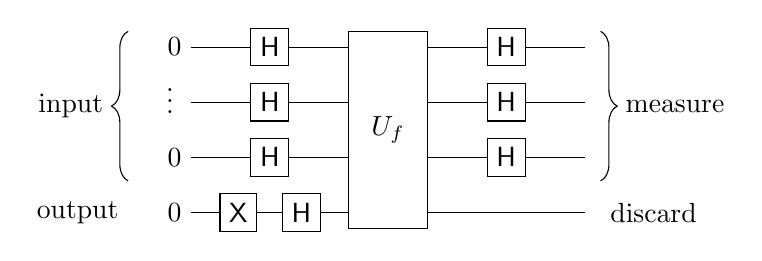
\begin{tikzpicture}
    \addstate{$\bket{0}$}{0}{5};
    \addstate{$\rvdots\;$}{1}{5};
    \addstate{$\bket{0}$}{2}{5};
    \addstate{$\bket{0}$}{3}{5};
    \addoperator{$\qH$}{0}{1};
    \addoperator{$\qH$}{1}{1};
    \addoperator{$\qH$}{2}{1};
    \addoperator{$\qX$}{3}{0.6};
    \addoperator{$\qH$}{3}{1.4};
    \addbigoperator{$U_f$}{0}{3}{2}{3};
    \addoperator{$\qH$}{0}{4};
    \addoperator{$\qH$}{1}{4};
    \addoperator{$\qH$}{2}{4};

    \draw [decorate, decoration={brace, amplitude=6pt}] (-0.8, -1.7) -- (-0.8, 0.2) node [pos=0.5, left] {input\;\;};

    \node [left] at (-0.8, -2.1) {output};

    \draw [decorate, decoration={brace, amplitude=6pt}] (5.2, 0.2) -- (5.2, -1.7) node [pos=0.5, right] {\;\;measure};

    \node [right] at (5.2, -2.1) {discard};
  \end{tikzpicture}
\end{center}
This uses exactly one query, with $1 + (n + 1) + n + n = O(n)$ elementary gates and measurements.

What if we tolerate error in the balanced vs constant problem? In other words, we only require that the answer is correct with probability $1 - \varepsilon$ with $0 < \varepsilon < \frac{1}{2}$.

In the quantum case, nothing much changes, since we are probably not going to do better than $1$ query. However, we no longer have a huge benefit over classical algorithms. There is a classical randomized algorithm with $O(\log(1/\varepsilon))$ queries, and in particular does not depend on $n$.

Indeed, we do it the obvious way --- we choose some $K$ $x$-values uniformly at random from $B_n$, say $x_1, \cdots, x_n$ (where $K$ is fixed and determined later). We then evaluate $f(x_1), \cdots, f(x_n)$.

If all the outputs are the same, then we say $f$ is constant. If they are not the same, then we say $f$ is balanced.

If $f$ actually is constant, then the answer is correct with probability $1$. If $f$ is balanced, then each $f(x_i)$ is $0$ or $1$ with equal probability. So the probability of getting the same values for all $x_i$ is
\[
  \frac{2}{2^K} = 2^{1 - K}.
\]
This is our failure probability. So if we pick
\[
  K > \log_2 (\varepsilon^{-1}) + 1,
\]
then we have a failure probability of less than $\varepsilon$.

Can we decide \emph{every} yes/no question about $f: B_n \to B_1$'s by quantum algorithms with ``a few'' queries? The answer is no. One prominent example is the \term{SAT problem} (\term{satisfiability problem}) --- given an arbitrary $f$, we want to determine if there an $x$ such that $f(x) = 1$? It can be shown that any quantum algorithm (even if we allow for bounded errors) needs at least $O(\sqrt{2^n})$ queries, which is achieved by Grover's algorithm. Classically, we need $O(2^n)$ queries. So we have achieved a square root speedup, which is good, but not as good as the Deutsch-Jozsa algorithm.

In any case, the Deutsch-Jozsa algorithm demonstrates how we can achieve an exponential benefit with quantum algorithms, but it happens only when we have no error tolerance. In real life scenario, external factors will lead to potential errors anyway, and requiring that we are always correct is not a sensible requirement.

There are other problems where quantum algorithms are better:
\begin{eg}[Simon's algorithm]\index{Simon's algorithm}
  The \term{Simon's problem} is a promise problem about $f: B_n \to B_n$ with provably exponential separation between classical ($O(2^{n/4})$) and quantum ($O(n)$) query complexity even with bounded error. The details are on the first example sheet.
\end{eg}

\subsection{Quantum Fourier transform and periodicities}
We've just seen some nice examples of benefits of quantum algorithms. However, oracles are rather unnatural problems --- it is rare to just have a black-box access to a function without knowing anything else about the function.

How about more ``normal'' problems? The issue with trying to compare quantum and classical algorithms for ``normal'' problems is that we don't actually have any method to find the lower bound for the computation complexity. For example, while we have not managed to find polynomial prime factorization algorithms, we cannot prove for sure that there isn't any classical algorithm that is polynomial time. However, for the prime factorization problem, we \emph{do} have a quantum algorithm that does much better than all known classical algorithms. This is \emph{Shor's algorithm}, which relies on the toolkit of the quantum Fourier transform.

We start by defining the quantum Fourier transform.
\begin{defi}[Quantum Fourier transform mod $N$]\index{quantum Fourier transform}
  Suppose we have an $N$-dimensional state space with basis $\bket{0}, \bket{1}, \cdots, \bket{N - 1}$ labelled by $\Z/N\Z$. The \emph{quantum Fourier transform mod $N$} is defined by
  \[
    \qQFT: \bket{a} \mapsto \frac{1}{\sqrt{N}} \sum_{b = 0}^{N - 1} e^{2\pi i ab/N} \bket{b}.
  \]
  The matrix entries are
  \[
    [\qQFT]_{ab} = \frac{1}{\sqrt{N}} \omega^{ab},\quad \omega = e^{2\pi i/N},
  \]
  where $a, b = 0, 1, \cdots, N - 1$. We write \term{$\qQFT_n$} for the quantum Fourier transform mod $n$.
\end{defi}
Note that we are civilized and start counting at $0$, not $1$.

We observe that the matrix $\sqrt{N}\qQFT$ is
\begin{enumerate}
  \item Symmetric
  \item The first (i.e.\ $0$th) row and column are all $1$'s.
  \item Each row and column is a geometric progression $1, r, r^2, \cdots, r^{n - 1}$, where $r = \omega^k$ for the $k$th row or column.
\end{enumerate}

\begin{eg}
  If we look at $\qQFT_2$, then we get our good old $\qH$. However, $\qQFT_4$ is not $H \otimes H$.
\end{eg}

\begin{prop}
  $\qQFT$ is unitary.
\end{prop}

\begin{proof}
  We use the fact that
  \[
    1 + r + \cdots + r^{N - 1} =
    \begin{cases}
      \frac{1 - r^N}{1 - r} & r \not= 1\\
      N & r = 1
    \end{cases}.
  \]
  So if $r = \omega^k$, then we get
  \[
    1 + r + \cdots + r^{N - 1} =
    \begin{cases}
      0 & k \not\equiv 0 \mod N\\
      N & k \equiv 0 \mod N
    \end{cases}.
  \]
  Then we have
  \[
    (\qQFT^\dagger \qQFT)_{ij} = \frac{1}{\sqrt{N}^2} \sum_k \omega^{-ik} \omega^{jk} =\frac{1}{N} \sum_k \omega^{(j-i)k} =
    \begin{cases}
      1 & i = j\\
      0 & i \not= j
    \end{cases}.\qedhere
  \]
\end{proof}

We now use the quantum Fourier Transform to solve the periodicity problem.
\begin{eg}\index{Periodicity problem}
  Suppose we are given $f: \Z/N\Z \to Y$ (for some set $Y$). We are promised that $f$ is periodic with some period $r \mid N$, so that
  \[
    f(x + r) = f(x)
  \]
  for all $x$. We also assume that $f$ is injective in each period, so that
  \[
    0 \leq x_1 \not= x_2 \leq r - 1\quad\text{ implies }\quad f(x_1) \not= f(x_2).
  \]
  The problem is to find $r$, with any constant level of error $1 - \varepsilon$ independent of $N$. Since this is not a decision problem, we can allow $\varepsilon > \frac{1}{2}$.

  In the classical setting, if $f$ is viewed as an oracle, then $O(\sqrt{N})$ queries are necessary and sufficient. We are going to show that quantumly, $O(\log \log N)$ queries with $O(\mathrm{poly}(\log N))$ processing steps suffice. In later applications, we will see that the relevant input size is $\log N$, not $N$. So the classical algorithm is exponential time, while the quantum algorithm is polynomial time.

  Why would we care about such a problem? It turns out that later we will see that we can reduce prime factorization into a periodicity problem. While we will actually have a very explicit formula for $f$, there isn't much we can do with it, and treating it as a black box and using a slight modification of what we have here will be much more efficient than any known classical algorithm.

  The quantum algorithm is given as follows:
  \begin{enumerate}
    \item Make $\frac{1}{\sqrt{N}} \sum_{x = 0}^{N - 1} \bket{x}$. For example, if $N = 2^n$, then we can make this using $\qH \otimes \cdots \otimes \qH$. If $N$ is not a power of $2$, it is not immediately obvious how we can make this state, but we will discuss this problem later.

    \item We make one query to get
      \[
        \bket{f} = \frac{1}{\sqrt{N}} \sum \bket{x} \bket{f(x)}.
      \]

    \item We now recall that $r \mid N$, Write $N = Ar$, so that $A$ is the number of periods. We measure the second register, and we will see some $y = f(x)$. We let $x_0$ be the \emph{least} $x$ with $f(x) = y$, i.e.\ it is in the first period. Note that we don't know what $x_0$ is. We just know what $y$ is.

      By periodicity, we know there are exactly $A$ values of $x$ such that $f(x) = y$, namely
      \[
        x_0,\, x_0 + r,\, x_0 + 2r,\, \cdots,\, x_0 + (A - 1)r.
      \]
      By the Born rule, the first register is collapsed to
      \[
        \bket{\mathrm{per}} = \left(\frac{1}{\sqrt{A}} \sum_{j = 0}^{A - 1} \bket{x_0 + jr}\right) \bket{f(x_0)}.
      \]
      We throw the second register away. Note that $x_0$ is chosen randomly from the first period $0, 1, \cdots, r - 1$ with equal probability.

      What do we do next? If we measure $\bket{\mathrm{per}}$, we obtain a random $j$-value, so what we actually get is a random element ($x_0$th) of a random period ($j$th), namely a uniformly chosen random number in $0, 1, \cdots, N$. This is not too useful.

    \item The solution is the use the quantum Fourier transform, which is not surprising, since Fourier transforms are classically used to extract periodicity information.

      Apply $\qQFT_N$ to $\bket{\mathrm{per}}$ now gives
      \begin{align*}
        \qQFT_N \bket{\mathrm{per}} &= \frac{1}{\sqrt{NA}} \sum_{j = 0}^{n - 1} \sum_{y = 0}^{N - 1} \omega^{(x_0 + jr) y} \bket{y}\\
        &= \frac{1}{\sqrt{NA}} \sum_{y = 0}^{N - 1} \omega^{x_0 y}\left(\sum_{j = 0}^{n - 1}\omega^{jry}\right) \bket{y}
      \end{align*}
      We now see the inner sum is a geometric series. If $\omega^{ry} = 1$, then this sum is just $A$. Otherwise, we have
      \[
        \sum_{j = 0}^{A - 1} \omega^{jry} = \frac{1 - \omega^{rA}}{1 - \omega^{ry}} = \frac{1 - 1}{1 - \omega^{ry}} = 0.
      \]
      So we are left with
      \[
        \qQFT_n \bket{\mathrm{per}} = \sqrt{\frac{A}{N}} \sum_{k = 0}^{r - 1}\omega ^{x_0 k N/r} \bket{k\frac{N}{r}}.
      \]
      Note that before the Fourier transform, the random shift of $x_0$ lied in the label $\bket{x_0 + jr}$. After the Fourier transform, it is now encoded in the phase instead.

    \item Now we can measure the label, and we will get some $C$ which is a multiple $k_0 \frac{N}{r}$, where $0 \leq k_0 \leq r - 1$ is chosen uniformly at random. We rewrite this equation as
      \[
        \frac{k_0}{r} = \frac{C}{N}.
      \]
      We know $C$, because we just measured it, and $N$ is a given in the question. Also, $k_0$ is randomly chosen, and $r$ is what we want. So how do we extract that out?

      If by good chance, we have $k_0$ coprime to $r$, then we can cancel $C/N$ to lowest terms and read off $r$ as the resulting denominator $\tilde{r}$. Note that cancelling $C/N$ to lowest terms can be done quickly by Euclidean algorithm. But how likely are we to be so lucky? We can just find some number theory book, and figure out that the number of natural numbers $< r$ that are coprime to $r$ grows as $O(r/\log \log r)$. More precisely, it is $\sim e^{-\gamma} r/\log \log r$, where $\gamma$ is the other Euler's constant. We note that
      \[
        O\left(\frac{r}{\log \log r}\right) > O\left(\frac{1}{\log \log N}\right).
      \]
      So if $k_0$ is chosen uniformly and randomly, the probability that $k_0$ is coprime to $r$ is at least $O(1/\log \log N)$.

      Note that if $k_0$ is \emph{not} coprime with $r$, then we have $\tilde{r} \mid r$, and in particular $\tilde{r} < r$. So we can check if $\tilde{r}$ is a true period --- we compute $f(0)$ and $f(\tilde{r})$, and see if they are the same. If $\tilde{r}$ is wrong, then they cannot be equal as $f$ is injective in the period.

      While the probability of getting a right answer decreases as $N \to \infty$, we just have to do the experiment many times. From elementary probability, if an event has some (small) success probability $p$, then given any $0 < 1 - \varepsilon < 1$, for $M = - \frac{\log \varepsilon}{p}$ trials, the probability that there is at least one success is $ > 1 - \varepsilon$. So if we repeat the quantum algorithm $O(\log \log N)$ times, and check $\tilde{r}$ each time, then we can get a true $r$ with any constant level of probability.
    \item We can further improve this process --- if we have obtained two attempts $\tilde{r}, \tilde{r}'$, then we know $r$ is at least their least common multiple. So we can in fact achieve this in constant time, if we do a bit more number theory. However, the other parts of the algorithm (e.g.\ cancelling $C/N$ down to lowest terms) still use time polynomial in $\log N$. So we have a polynomial time algorithm.
  \end{enumerate}
\end{eg}

There is one thing we swept under the carpet. We need to find an efficient way of computing the quantum Fourier transform, or else we just hid all our complexity in the quantum Fourier transform.

In general, we would expect that a general unitary operations on $n$ qubits needs $\exp(n)$ elementary circuits. However, the quantum Fourier transform is special.

\begin{fact}
  $\qQFT_{2^n}$ can be implemented by a quantum circuit of size $O(n^2)$.
\end{fact}
The idea of the construction is to mimic the classical fast Fourier transform. An important ingredient of it is:
\begin{fact}
  The state
  \[
    \qQFT_{2^n} \bket{x} = \frac{1}{2^{n/2}} \sum_{y = 0}^{2^n - 1} \omega^{xy}\bket{y}
  \]
  is in fact a product state.
\end{fact}
We will not go into the details of implementation.

We can generalize the periodicity problem to arbitrary groups, known as the \term{hidden subgroup problem}. We are given some oracle for $f: G \to Y$, and we are promised that there is a subgroup $H < G$ such that $f$ is constant and distinct on cosets of $H$ in $G$. We want to find $H$ (we can make ``find'' more precise in two ways --- we can either ask for a set of generators, or provide a way of sampling uniformly from $H$).

In our case, we had $G = (\Z/N\Z, +)$, and our subgroup was
\[
  H = \{0, r, 2r, \cdots, (A - 1) r\}.
\]
Unfortunately, we do not know how to do this efficiently for a group in general.

\subsection{Shor's algorithm}
All that was a warm up for \emph{Shor's algorithm}. This is a quantum algorithm that factorizes numbers in polynomial time. The crux of the algorithm will be a modified version of the quantum Fourier transform.

The precise statement of the problem is as follows --- given an integer $N$ with $n = \log N$ digits, we want to find a factor $1 < K < N$. Shor's algorithm will achieve this with constant probability $(1 - \varepsilon)$ in $O(n^3)$ time. The best known classical algorithm is $e^{O(n^{1/3} (\log n)^{2/3})}$.

To do this, we will use the periodicity algorithm. However, there is one subtlety involved. Instead of working in $\Z/n\Z$, we need to work in $\Z$. Since computers cannot work with infinitely many numbers, we will have to truncate it somehow. Since we have no idea what the period of our function will be, we must truncate it randomly, and we need to make sure we can control the error introduced by the truncation.

We shall now begin. Given an $N$, we first choose some $1 < a < N$ uniformly randomly, and compute $\hcf(a, N)$. If it is not equal to $1$, then we are finished. Otherwise, by Euler's theorem, there is a least power $r$ of $a$ such that $a^r \equiv 1 \bmod N$. The number $r$ is called the \emph{order} of $a$ mod $N$. It follows that the function $f: \Z \to \Z/N\Z$ given by $f(k) = a^k \bmod N$ has period $r$, and is injective in each period.

Note that $f(k)$ can be efficiently computed in $\poly(\log k)$ time, by repeated squaring. Also note that classically, it is hard to find $r$, even though $f$ has a simple formula!

It was known to Legendre in 1800 that knowing $r$ means we can factor $n$. Suppose we can find $r$, and further suppose $r$ is even. Then we have
\[
  a^r - 1 \equiv (a^{r/2} + 1)(a^{r/2} - 1) \equiv 0 \pmod N.
\]
So $N$ exactly divides the product. By minimality of $r$, we know $N$ does not divide $a^{r/2} - 1$. So if $N$ does not divide $a^{r/2} + 1$ as well, then $\hcf(N, a^{r/2} \pm 1)$ are non-trivial factors of $N$.

For this to work, we needed two assumptions -- $r$ is even, and $a^{r/2} \not\equiv -1 \pmod N$. Fortunately, there is a theorem in number theory that says if $N$ is odd and not a prime power, and $a$ is chosen uniformly at random, then the probability that these two things happen is at least $\frac{1}{2}$. In fact, it is $\geq 1 - \frac{1}{2^{m - 1}}$, where $m$ is the number of prime factors of $N$.

So if we repeat this $k$ times, the probability that they all fail to give a factor is less than $\frac{1}{2^k}$. So this can be as small as we wish.

What about the other possibilities? If $N$ is even, then we would have noticed by looking at the last digit, and we can just write down $2$. If $N = c^\ell$ for $c, \ell > 2$, then there is a classical polynomial time algorithm that outputs $c$, which is a factor. So these are the easy cases.

Everything we've done so far is classical! The quantum part comes in when we want to compute $r$. We know that $f(k) = a^k$ is periodic on $\Z$, which is an infinite domain. So we cannot just apply our periodicity algorithm.

By number theory, we know that $r$ is at most $N$. But other than that, we have no idea what $r$ actually is, nor do we know of any multiple of $r$. So we cannot apply the periodicity argument directly. Instead, we pick a big number $2^m$, and work on the domain $D = \{0, 1, \cdots, 2^m - 1\} = \Z/2^m \Z$. How do we choose $m$? The idea is that we want $0, \cdots, 2^m - 1$ to contain $B$ full periods, plus some extra ``corrupt'' noise $b$, so
\[
  2^m = Br + b,
\]
with $0 \leq b < r$. Since we want to separate out the periodicity information from the corrupt noise, we will want $b$ to be relatively small, compared to $Br$. We know the size of $b$ is bounded by $r$, hence by $N$. So we need $2^m$ to be ``much larger'' than $N$. It turns out picking $2^m > N^2$ is enough, and we will pick $m$ to be the smallest number such that this holds.

We now study the effect of corruption on the periodicity algorithm. We again make the state
\[
  \bket{f} = \frac{1}{\sqrt{2^m}} \sum \bket{x} \bket{f(x)}.
\]
and measure the value of $f$. We then get
\[
  \bket{\mathrm{per}} = \frac{1}{\sqrt{A}} \sum_{k = 0}^{A - 1} \bket{x_0 + kr},
\]
where $A = B$ or $B + 1$, depending on whether $x_0 \leq b$ or not. As before, we apply $\qQFT_{2^m}$ to obtain
\[
  \qQFT_{2^m}\bket{\mathrm{per}} = \sum_{c = 0}^{2^n - 1} \tilde{f}(c) \bket{c}.
\]
When we did this before, with an exact period, most of the $\hat{f}(c)$ is zero. However, this time things are a bit more messy. As before, we have
\[
  \tilde{f}(c) = \frac{\omega^{c x_0}}{\sqrt{A}\sqrt{2^m}} [1 + \alpha + \cdots + \alpha^{A - 1}],\quad \alpha = e^{2\pi i cr/2^m}.
\]
The important question is, when we measure this, which $c$'s will we see with ``good probability''? With exact periodicity, we knew that $\frac{2^m}{r} = A$ is an exact integer. So $\tilde{f}(c) = 0$ except when $c$ is a multiple of $A$. Intuitively, we can think of this as interference, and we had totally destructive and totally constructive interference respectively.

In the inexact case, we will get constructive interference for those $c$ such that the phase $\alpha$ is close to $1$. These are the $c$'s with $\frac{cr}{2^m}$ nearest to integers $k$, and the powers up to $\alpha^{A - 1}$ don't spread too far around the unit circle. So we avoid cancellations.

So we look at those special $c$'s having this particular property. As $c$ increases from $0$ to $2^m - 1$, the angle $\frac{cr}{2^m}$ increments by $\frac{r}{2^m}$ each time from $0$ up to $r$. So we have $c_k$'s for each $k = 0, 1, \cdots, r - 1$ such that
\[
  \left|\frac{c_k r}{2^m} - k\right| < \frac{1}{2} \cdot \frac{r}{2^m}.
\]
In other words, we have
\[
  \left|c_k - k\frac{2^m}{r}\right| < \frac{1}{2}.
\]
So the $c_k$ are the integers nearest to the multiples of $2^m/r$.

In $\tilde{f}(c)$, the $\alpha$'s corresponding to the $c_k$'s have the smallest phases, i.e.\ nearest to the positive real axis. We write
\[
  \frac{c_k r}{2^m} = k + \xi,
\]
where
\[
  k \in \Z,\quad |\xi| < \frac{1}{2} \frac{r}{2^m}.
\]
Then we have
\[
  \alpha^n = \exp\left(2\pi i \frac{c_k r}{2^m}n\right) = \exp\left(e\pi i(k + \xi)n\right) = \exp(2 \pi i \xi n)
\]
Now for $n < A$, we know that $|2 \xi n| < \pi$, and thus $1, \alpha, \alpha^2, \cdots, \alpha^{A - 1}$ all lie in the lower half plane or upper half plane.

Doing all the algebra needed, we find that if $\qQFT\bket{\mathrm{per}}$ is measured, then for any $c_k$ as above, we have
\[
  \mathrm{Prob}(c_k) > \frac{\gamma}{r},
\]
where
\[
  \gamma = \frac{4}{\pi^2} \approx 0.4.
\]
Recall that in the exact periodicity case, the points $c_k$ hit the integers exactly, and instead of $\gamma$ we had $1$. The distribution of the $c$'s then look like:
\begin{center}
  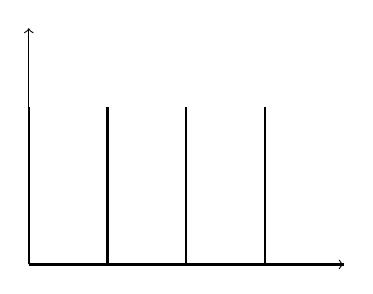
\begin{tikzpicture}
    \draw [->] (0, 0) -- (4, 0);
    \draw [->] (0, 0) -- (0, 3);

    \foreach \x in {0, 1, 2, 3} {
      \draw [thick] (\x, 0) -- (\x, 2);
    }
    \draw [thick] (0, 0) -- (4, 0);
  \end{tikzpicture}
\end{center}
With inexact periods, we obtain something like
\begin{center}
  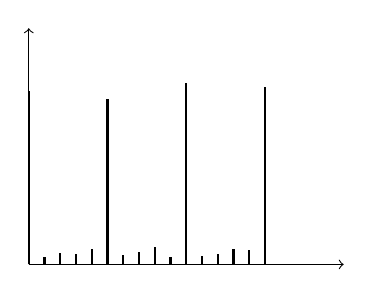
\begin{tikzpicture}
    \draw [->] (0, 0) -- (4, 0);
    \draw [->] (0, 0) -- (0, 3);

    \foreach \x/\y in {0/2.2, 1/2.1, 2/2.3, 3/2.25} {
      \draw [thick] (\x, 0) -- (\x, \y);
    }
    \foreach \x\y in {0.2/0.1,0.4/0.15,0.6/0.13,0.8/0.2,1.2/0.12,1.4/0.16,1.6/0.22,1.8/0.09,2.2/0.11,2.4/0.13,2.6/0.2,2.8/0.18} {
      \draw [thick] (\x, 0) -- (\x, \y);
    }
  \end{tikzpicture}
\end{center}
Now how do we get $r$ from a $c_k$? We know
\[
  \left| \frac{c_k}{2^m} - \frac{k}{r}\right| < \frac{1}{2^{m + 1}} < \frac{1}{2N^2}.
\]
We claim that there is at most 1 fraction $\frac{k}{r}$ with denominator $< N$ such that this inequality holds. So this inequality does uniquely determine $k/r$.

Indeed, suppose $\frac{k}{r}$ and $\frac{k'}{r'}$ both work. Then we have
\[
  \left|\frac{k'}{r'} - \frac{k}{r}\right| = \frac{|k'r - r'k|}{rr'} > \frac{1}{rr'} > \frac{1}{N^2}.
\]
However, we also have
\[
  \left|\frac{k'}{r'} - \frac{k}{r}\right| \leq \left|\frac{k'}{r'} - \frac{c_k}{2^m}\right| + \left|\frac{c_k}{2^m} - \frac{k}{r}\right| < \frac{1}{2N^2} + \frac{1}{2N^2} = \frac{1}{N^2}.
\]
So it follows that we must have $\frac{k'}{r'} = \frac{k}{r}$.

We introduce the notion of a ``good'' $c_k$ value, which is when $k$ is coprime to $r$. The probability of getting a good $c_k$ is again
\[
  O(1/\log \log r) > O(1/\log \log N).
\]
Note that this is the same rate as the case of exact periodicity, since we have only lost a constant factor of $\gamma$! If we did have such a $c_k$, then now $r$ is uniquely determined.

However, there is still the problem of finding $r$ from a good $c_k$ value. At this point, this is just classical number theory.

We can certainly try all $\frac{k'}{r'}$ with $k' < r' < N$ and find the closest one to $c_k/2^m$, but there are $O(N^2)$ fractions to try, but we want a $O(\mathrm{poly}(\log N))$ algorithm. Indeed, if we were to do it this way, we might as well try all numbers less than $N$ and see if they divide $N$. And this is just $O(N)$!

The answer comes from the nice theory of continued fractions. Any rational number $\frac{s}{t} < 1$ has a continued fraction expansion
\[
  \frac{s}{t} = \cfrac{1}{a_1 + \cfrac{1}{a_2 + \cfrac{1}{a_3 + \cdots}}}.
\]
Indeed to do this, we simply write
\[
  \frac{s}{t} = \cfrac{1}{\cfrac{t}{s}} = \cfrac{1}{a_1 + \cfrac{s_1}{t_1}},
\]
where we divide $t$ by $s$ to get $t = a_1s + s_1$, and then put $t_1 = s$. We then keep going on with $\frac{s_1}{t_1}$. Since the numbers $s_i, t_i$ keep getting smaller, it follows that this process will eventually terminate.

Since it is very annoying to type these continued fractions in \LaTeX, we often write the continued fraction as
\[
  \frac{s}{t} = [a_1, a_2, a_3, \cdots, a_n].
\]
We define the $k$th convergent of $\frac{s}{t}$ to be
\[
  \frac{p_k}{q_k} = [a_1, a_2, \cdots, a_k].
\]
There are some magic results from number theory that gives us a simple recurrence relation for the convergents.
\begin{lemma}
  For $a_1, a_2, \cdots, a_\ell$ any positive reals, we set
  \begin{align*}
    p_0 &= 0 & q_0 &= 1\\
    p_1 &= 1 & q_1 &= a_1
  \end{align*}
  We then define
  \begin{align*}
    p_k &= a_k p_{k - 1} + p_{k - 2}\\
    q_k &= a_k q_{k - 1} + q_{k - 2}
  \end{align*}
  Then we have
  \begin{enumerate}
    \item We have
      \[
        [a_1, \cdots, a_k] = \frac{p_k}{q_k}.
      \]
    \item We also have
      \[
        q_k p_{k - 1} - p_k q_{k - 1} = (-1)^k.
      \]
      In particular, $p_k$ and $q_k$ are coprime.
  \end{enumerate}
\end{lemma}

From a bit more number theory, we find that
\begin{fact}
  If $s < t$ are $m$-bit integers, then the continued fraction has length $O(m)$, and all convergents $\frac{p_k}{q_k}$ can be computed in $O(m^3)$ time.
\end{fact}

More importantly, we have the following result:
\begin{fact}
  Let $0 < x < 1$ be rational, and suppose $\frac{p}{q}$ is rational with
  \[
    \left|x - \frac{p}{q}\right| < \frac{1}{2q^2}.
  \]
  Then $\frac{p}{q}$ is a convergent of the continued fraction of $x$.
\end{fact}

Then by this theorem, for a good $c$, we know $\frac{k}{r}$ must be a convergent of $\frac{c}{2^m}$. So we compute all convergents find a (unique) one whose denominator is less than $N$ and is within $\frac{1}{2N^2}$ of $\frac{c}{2^m}$. This gives us the value of $r$, and we are done.

In fact, this last classical part is the slowest part of the algorithm.

\begin{eg}
  Suppose we want to factor $N = 39$. Suppose the random $a$ we chose is $a = 7 < 39$, which is coporime to $N$. Let $r$ be the period of $f(x) = 7^x \bmod 39$.

  We notice
  \[
    1024 = 2^{10} < N^2 = 1621 < 2^{11} = 2048.
  \]
  So we pick $m = 11$. Suppose the measurement of $\qQFT_{2^m}\bket{\mathrm{per}}$ yeilds $c = 853$.

  By the theory, this has a constant probability (approximately $0.4$) to satisfy
  \[
    \left|\frac{853}{2^m} - \frac{k}{r}\right| < \frac{1}{2^{m + 1}} = \frac{1}{2^{12}} < \frac{1}{2N^2}.
  \]
  We also have a probability of $O(1/\log \log r)$ to have $k$ and $r$ coprime. In this case, $c$ is indeed ``good''. So there is a unique $\frac{k}{r}$ satisfying
  \[
    \left|\frac{853}{2048} - \frac{k}{r}\right| < \frac{1}{2^{12}}.
  \]
  So to find $\frac{k}{r}$, we do the continued fraction expansion of $\frac{853}{2048}$. We have
  \[
    \frac{853}{2048} = \cfrac{1}{\cfrac{2048}{853}} = \cfrac{1}{2 + \cfrac{342}{853}} = \cfrac{1}{2 + \cfrac{1}{\cfrac{853}{342}}} = \cfrac{1}{2 + \cfrac{1}{2 + \cfrac{169}{342}}} = \cdots = [2, 2, 2, 42, 4].
  \]
  We can then compute the convergents
  \begin{align*}
    [2] &= \frac{1}{2}\\
    [2, 2] &= \frac{2}{5}\\
    [2, 2, 2] &= \frac{5}{12}\\
    [2, 2, 2, 42] &= \frac{212}{509}\\
    [2, 2, 2, 42, 4] &= \frac{853}{2048}
  \end{align*}
  Of all these numbers, only $\frac{5}{12}$ is within $\frac{1}{2^{12}}$ of $\frac{853}{2048}$ and whose denominator is less than $N = 39$.

  If we do not assume $k$ and $r$ are coprime, then the possible $\frac{k}{r}$ are
  \[
    \frac{5}{12}, \frac{10}{24}, \frac{15}{36}.
  \]
  If we assume that $\frac{k}{r}$ are coprime, then $r = 12$. Indeed, we can try that
  \[
    7^{12} \equiv 1 \pmod {39}.
  \]
  So we now know that
  \[
    39 \mid (7^6 + 1)(7^6 - 1).
  \]
  We now hope/expect with probability $>\frac{1}{2}$ exactly that it goes partly into each factor. We can compute
  \begin{align*}
    7^6 + 1 &= 117650 \equiv 26 \pmod {39}\\
    7^6 - 1 &= 117648 \equiv 24 \pmod {39}
  \end{align*}
  We can then compute
  \[
    \hcf(26, 39) = 13,\quad \hcf(24, 39) = 3 \pmod {39}.
  \]
  We see that $3$ and $13$ are factors of $39$.
\end{eg}

\subsection{Search problems and Grover's algorithm}
We are now going to turn our attention to search problems. These are very important problems in computing, as we can formulate almost all problems as some sort of search problems.

One important example is simultaneous constraint satisfaction. Here we have a large configuration space of options, and we want to find some configuration that satisfies some constraints. For example, when designing a lecture timetable for Part III courses, we need to schedule the courses so that we don't clash two popular courses in the same area, and the courses need to have big enough lecture halls, and we have to make sure a lecturer doesn't have to simultaneously lecture two courses at the same time. This is very complicated.

In general, search problems have some common features:
\begin{enumerate}
  \item Given any instance of solution attempt, it is easy to check if it is good or not.
  \item There are exponentially many possible instances to try out.
\end{enumerate}

One example is the boolean satisfiability problem, which we have already seen before.
\begin{eg}[Boolean satisfiability problem]
  The \term{boolean satisfiability problem} (\term{SAT}) is as follows --- given a Boolean formula $f: B_n \to B$, we want to know if there is a ``satisfying argument'', i.e.\ if there is an $x$ with $f(x) = 1$.
\end{eg}

This has complexity class \textbf{NP}, standing for \emph{non-deterministic polynomial time}. There are many ways to define \textbf{NP}, and here we will provide two. The first definition of \textbf{NP} will involve the notion of a verifier:

\begin{defi}[Verifier]
  Suppose we have a language $L \subseteq B^*$, where
  \[
    B^* = \bigcup_{n \in \N} B_n
  \]
  is the set of all bit strings.

  A \term{verifier} for $L$ is a computation $V(w, c)$ with two inputs $w, c$ such that
  \begin{enumerate}
    \item $V$ halts on all inputs.
    \item If $w \in L$, then for \emph{some} $c$, $V(w, c)$ halts with ``accept''.
    \item If $w \not\in L$, then for \emph{all} $c$, $V(w, c)$ halts with ``reject''.
  \end{enumerate}
  A \term{polynomial time verifier} is a $V$ that runs in polynomial time in $|w|$ (not $|w| + |c|!$).
\end{defi}
We can think of $c$ as ``certificate of membership''. So if you are a member, you can exhibit a certificate of membership that you are in there, and we can check if the certification is valid. However, if you are not a member, you cannot ``fake'' a certificate.

\begin{defi}[Non-deterministic polynomial time problem]\index{\textbf{NP}}\index{non-deterministic polynomial time}
  \textbf{NP} is the class of languages that have polynomial time verifiers.
\end{defi}

\begin{eg}
  The SAT problem is in \textbf{NP}. Here $c$ is the satisfying argument, and $V(f, c)$ just computes $f(c)$ and checks whether it is $1$.
\end{eg}

\begin{eg}
  Determining if a number is composite is in \textbf{NP}, where a certificate is a factor of the number.
\end{eg}
However, it is not immediately obvious that testing if a number is prime is in \textbf{NP}. It is an old result that it indeed is, and recent progress shows that it is in fact in \textbf{P}.

It is rather clear that $\mathbf{P} \subseteq \mathbf{NP}$. Indeed, if we can check membership in polynomial time, then we can also construct a verifier in polynomial time that just throws the certificate away and check directly.

There is another model of \textbf{NP}, via \term{non-deterministic computation}. Recall that in probabilistic computation, in some steps, we had to pick a random number, and picking a different number would lead to a different ``branch''. In the case of non-deterministic computation, we are allowed to take \emph{all} paths at the same time. If \emph{some} of the paths end up being accepting, then we accept the input. If \emph{all} paths reject, then we reject the input. Then we can alternatively say a problem is in \textbf{NP} if there is a polynomial-time non-deterministic machine that checks if the string is in the language.

It is not difficult to see that these definitions of \textbf{NP} are equivalent. Suppose we have a non-deterministic machine that checks if a string is in the language. Then we can construct a verifier whose certificate is a prescription of which particular branch we should follow. Then the verifier just takes the prescription, follows the path described and see if we end up being accepted.

Conversely, if we have a verifier, we can construct a non-deterministic machine by testing a string on \emph{all} possible certificates, and check if any of them accepts.

Unfortunately, we don't know anything about how these different complexity classes compare. We clearly have $\mathbf{P} \subseteq \mathbf{BPP} \subseteq \mathbf{BQP}$ and $\mathbf{P} \subseteq \mathbf{NP}$. However, we do not know if these inclusions are strict, or how $\mathbf{NP}$ compares to the others.

\subsubsection*{Unstructured search problem and Grover's algorithm}
Usually, when we want to search something, the search space we have is structured in some way, and this greatly helps our searching problem.

For example, if we have a phone book, then the names are ordered alphabetically. If we want to find someone's phone number, we don't have to look through the whole book. We just open to the middle of the book, and see if the person's name is before or after the names on the page. By one lookup like this, we have already eliminated half of the phone book we have to search through, and we can usually very quickly locate the name.

However, if we know someone's phone number and want to figure out their name, it is pretty much hopeless! This is the problem with unstructured data!

So the problem is as follows: we are given an unstructured database with $N = 2^n$ items and a \emph{unique} good item (or no good items). We can query any item for good or bad-ness. The problem is to find the good item, or determine if one exists.

Classically, $O(N)$ queries are necessary and sufficient. Even if we are asking for a right result with fixed probability $c$, if we pick items randomly to check, then the probability of seeing the ``good'' one in $k$ queries is given by $k/N$. So we still need $O(N)$ queries for any fixed probability.

Quantumly, we have \term{Grover's algorithm}. This needs $O(\sqrt{N})$ queries, and this is both necessary and sufficient.

The database of $N = 2^n$ items will be considered as an oracle $f: B_n \to B_1$. it is promised that there is a unique $x_0 \in B_n$ with $f(x_0) = 1$. The problem is to find $x_0$. Again, we have the quantum version
\[
  U_f \bket{x}\bket{y} = \bket{x} \bket{y \otimes f(x)}.
\]
However, we'll use instead $I_{x_0}$ on $n$ qubits given by
\[
  I_{x_0}\bket{x} =
  \begin{cases}
    \bket{x} & x \not= x_0\\
    -\bket{x} & x \not= x_0
  \end{cases}.
\]
This can be constructed from $U_f$ as we've done before, and one use of $I_{x_0}$ can be done with one use of $U_f$.
\begin{center}
  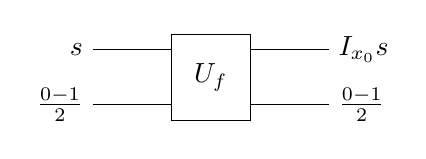
\begin{tikzpicture}
    \addstateend{$\bket{s}$}{0}{3} {$I_{x_0}\bket{s}$};
    \addstateend{$\frac{\bket{0} - \bket{1}}{2}$}{1}{3}{$\frac{\bket{0} - \bket{1}}{2}$};
    \addbigoperator{$U_f$}{0}{1}{1}{2};
  \end{tikzpicture}
\end{center}
We can write $I_{x_0}$ as
\[
  I_{x_0} = I - 2 \bket{x_0} \brak{x_0},
\]
where $I$ is the identity operator.

We are now going to state the \term{Grover's algorithm}, and then later prove that it works.

For convenience, we write
\[
  \qH_n = \underbrace{\qH \otimes \cdots \otimes \qH}_{n\text{ times}}
\]
We start with a uniform superposition
\[
  \bket{\psi_0} = \qH_n \bket{0\cdots0} = \frac{1}{\sqrt{n}} \sum_{\text{all }x} \bket{x}.
\]
We consider the \term{Grover iteration operator} on $n$ qubits given by
\[
  \mathcal{Q} = -\qH_n I_0 \qH_n I_{x_0}.
\]
Here running $I_{x_0}$ requires one query (whereas $I_0$ is ``free'' because it is just $I - 2 \bket{0}\brak{0}$).

Note that all these operators are all real. So we can pretend we are living in the real world and have nice geometric pictures of what is going on. We let $\mathcal{P}(x_0)$ be the (real) plane spanned by $\bket{x_0}$ and $\bket{\psi_0}$. We claim that
\begin{enumerate}
  \item In this plane $\mathcal{P}(x_0)$, this operator $\mathcal{Q}$ is a rotation by $2\alpha$, where
    \[
      \sin\alpha = \frac{1}{\sqrt{N}} = \braket{x_0}{\psi_0}.
    \]
  \item In the orthogonal complement $\mathcal{P}(x_0)^\perp$, we have $\mathcal{Q} = -I$.
\end{enumerate}
We will prove these later on. But if we know this, then we can repeatedly apply $\mathcal{Q}$ to $\bket{\psi_0}$ to rotate it near to $\bket{x_0}$, and then measure. Then we will obtain $\bket{x_0}$ with very high probability:
\begin{center}
  \begin{tikzpicture}
    \draw (0, 0) rectangle (5, 5);
    \node at (5, 5) [right] {$\mathcal{P}(x_0)$};
    \draw [->] (1, 1) -- (4, 1) node [right] {$\bket{\psi_0}$};
    \draw [dashed] (1, 1) -- (1, 4);
    \draw [->] (1, 1) -- (2, 4) node [above] {$\bket{x_0}$};

    \draw (1.4, 1) arc(0:71.57:0.4) node [pos=0.5, right] {$\beta$};
    \draw (1, 1.6) arc (90:71.57:0.6) node [pos=0.5, above] {$\alpha$};
  \end{tikzpicture}
\end{center}
The initial angle is
\[
  \cos \beta = \braket{x_0}{\psi_0} = \frac{1}{\sqrt{N}}.
\]
So the number of iterations needed is
\[
  \frac{\cos^{-1}(1/\sqrt{N})}{2 \sin^{-1}(1/\sqrt{N})} = \frac{\beta}{2\alpha}.
\]
In general, this is not an integer, but applying a good integer approximation to it will bring us to very close to $\bket{x_0}$, and thus we measure $x_0$ with high probability. For large $n$, the number of iterations is approximately
\[
  \frac{\pi/2}{2/\sqrt{N}} = \frac{\pi}{4} \sqrt{N}.
\]
\begin{eg}
  Let's do a boring example with $N = 4$. The initial angle satisfies
  \[
    \cos \beta = \frac{1}{\sqrt{4}} = \frac{1}{2}.
  \]
  So we know
  \[
    \beta = \frac{\pi}{3}.
  \]
  Similarly, we have
  \[
    2\alpha = 2 \sin^{-1}\frac{1}{2} = \frac{\pi}{3}.
  \]
  So $1$ iteration of $\mathcal{Q}$ will rotate $\bket{\psi_0}$ \emph{exactly} to $\bket{x_0}$, so we can find it with \emph{certainty} with 1 lookup.
\end{eg}
Now we prove that this thing actually works. In general, for any unitary $U$ and $I_{\bket{\psi}} = I - 2 \bket{\psi}\brak{\psi}$, we have
\[
  UI_{\bket{\psi}}U^\dagger = UIU^\dagger - 2U \bket{\psi} \brak{\psi} U^\dagger = I_{U \bket{\psi}}.
\]
In particular, since $H_n$ is self-adjoint, i.e.\ $H_n^\dagger H_n$, and that by definition $H_n \bket{0} = \bket{\psi_0}$, we know
\[
  \mathcal{Q} = -H_n I_0 H_n I_{x_0} = -I_{\bket{\psi_0}} I_{x_0}.
\]
Next we note that for any $\bket{\psi}$ and $\bket{\xi}$, we know by definition
\[
  I_{\bket{\psi}}\bket{\xi} = \bket{\xi} - 2 \bket{\psi} \braket{\psi}{\xi}.
\]
So this modifies $\bket{\xi}$ by some multiple of $\bket{\psi}$. So we know our operator
\[
  \mathcal{Q}\bket{\psi} = -I_{\bket{\psi_0}} I_{x_0}\bket{\psi}
\]
modifies $\bket{\psi}$ first by some multiple of $\bket{x_0}$, then by some multiple of $\psi_0$. So if $\bket{\xi} \in \mathcal{P}(x_0)$, then $\mathcal{Q} \bket{\psi} \in \mathcal{P}(x_0)$ too! So $\mathcal{Q}$ preserves $\mathcal{P}(x_0)$.

We know that $\mathcal{Q}$ is a unitary, and it is ``real''. So it must be a rotation or a reflection, since these are the only things in $\Or(2)$. We can explicitly figure out what it is. In the plane $\mathcal{P}(x_0)$, we know $I_{\bket{x_0}}$ is reflection in the mirror line perpendicular to $\bket{x_0}$. Similarly, $I_{\bket{\psi_0}}$ is reflection in the mirror line perpendicular to $\bket{\psi_0}$.

We now use the following facts about 2D Euclidean geometry:
\begin{enumerate}
  \item If $R$ is a reflection in mirror $M$ along $\bket{M}$, then $-R$ is reflection in mirror $M^\perp$ along $\bket{M^\perp}$.

    To see this, we know any vector can be written as $a\bket{M} + b \bket{M^\perp}$. Then $R$ sends this to $a \bket{M} - b\bket{M^\perp}$, while $-R$ sends it to $-a \bket{M} + b \bket{M^\perp}$, and this is reflection in $\bket{M^\perp}$.

  \item Suppose we have mirrors $M_1$ and $M_2$ making an angle of $\theta$:
    \begin{center}
      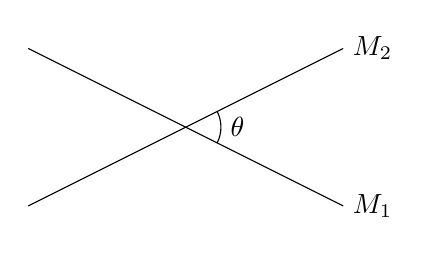
\begin{tikzpicture}
        \draw (-2, 1) -- (2, -1) node [right] {$M_1$};
        \draw (-2, -1) -- (2, 1) node [right] {$M_2$};
        \draw (0.4, -0.2) arc(-26.57:26.57:0.447) node [pos=0.5, right] {$\theta$};
      \end{tikzpicture}
    \end{center}
    Then reflection in $M_1$ then reflection in $M_2$ is the same as rotating counterclockwise by $2\theta$.
\end{enumerate}
So we know
\[
  \mathcal{Q} = -I_{\bket{\psi_0}} I_{\bket{x_0}}
\]
is reflection in $\bket{x_0^\perp}$ then reflection in $\bket{\psi_0^{\perp\perp}} = \bket{\psi_0}$. So this is a rotation by $2\alpha$, where $\alpha$ is the angle between $\bket{x_0^\perp}$ and $\bket{\psi_0}$, i.e.
\[
  \sin \alpha = \cos \beta = \braket{x_0}{\psi_0}.
\]
To prove our second claim that $\mathcal{Q}$ acts as $-\mathbf{1}$ in $\mathcal{P}(x_0)^\perp$, we simply note that if $\bket{\xi} \in \mathcal{P}(x_0)^\perp$, then $\bket{\xi} \perp \bket\psi_0$ and $\xi \perp\bket{x_0}$. So both $I_{\bket{x_0}}$ and $I_{\bket{\psi_0}}$ fix $\bket{\xi}$.

In fact, Grover's algorithm is the best algorithm we can achieve.
\begin{thm}
  Let $A$ be any quantum algorithm that solves the unique search problem with probability $1 - \varepsilon$ (for any constant $\varepsilon$), with $T$ queries. Then $T$ is at least $O(\sqrt{N})$. In fact, we have
  \[
    T \geq \frac{\pi}{4}(1 - \varepsilon) \sqrt{N}.
  \]
\end{thm}
So Grover's algorithm is not only optimal in the growth rate, but in the constant as well, asymptotically.

Proof is omitted.

\subsubsection*{Further generalizations}
Suppose we have multiple good items instead, say $r$ of them. We then replace $I_{x_0}$ with $I_f$, where
\[
  I_f \bket{x} =
  \begin{cases}
    -\bket{x} & x\text{ good}\\
    \bket{x} & x\text{ bad}
  \end{cases}
\]
We run the same algorithm as before. We let
\[
  \bket{\psi_{\mathrm{good}}} = \frac{1}{\sqrt{r}} \sum_{x\text{ good}} \bket{x}.
\]
Then now $\mathcal{Q}$ is a rotation through $2\alpha$ in the plane spanned by $\bket{\psi_{\mathrm{good}}}$ and $\bket{\psi_0}$ with
\[
  \sin \alpha = \braket{\psi_{\mathrm{good}}}{\psi_0} = \sqrt{\frac{r}{N}}.
\]
So for large $N$, we need
\[
  \frac{\pi/2}{2\sqrt{r/N}} = \frac{\pi}{4} \sqrt{\frac{N}{r}},
\]
i.e.\ we have a $\sqrt{r}$ reduction over the unique case. We will prove that these numbers are right later when we prove a much more general result.

What if we don't know what $r$ is? The above algorithm would not work, because we will not know when to stop the rotation. However, there are some tricks we can do to fix it. This involves cleverly picking angles of rotation at random, and we will not go into the details.

\subsection{Amplitude amplification}
In fact, the techniques from Grover's algorithm is completely general. Let $G$ be any subspace (``good'' subspace) of the state space $\mathcal{H}$, and $G^\perp$ be its orthogonal complement (``bad'' subspace). Then
\[
  \mathcal{H} = G \oplus G^\perp.
\]
Given any normalized vector $\bket{\psi} \in \mathcal{H}$, we have a unique decomposition with real, non-negative coefficients
\[
  \bket{\psi} = \sin \theta \bket{\psi_g} + \cos \theta \bket{\psi_b}
\]
such that
\[
  \bket{\psi_g} \in G,\quad \bket{\psi_b} \in G^\perp
\]
are normalized.

We define the reflections
\[
  I_{\bket{\psi}} = I -2\bket{\psi}\brak{\psi}, \quad I_g = I - 2P,
\]
where $P$ is the projection onto $G$ given by
\[
  P = \sum_b \bket{b}\brak{b}
\]
for any orthonormal basis $\{\bket{b}\}$ of $G$. This $P$ satisfies
\[
  P \bket{\psi} =
  \begin{cases}
    \bket{\psi} & \bket{\psi} \in G\\
    0 & \bket{\psi} \in G^\perp
  \end{cases}.
\]
We now define the \term{Grover operator}
\[
  \mathcal{Q} = - I_\psi I_G.
\]
\begin{thm}[Amplitude amplification thoerem]\index{amplitude amplification theorem}
  In the $2$-dimensional subspace spanned by $\bket{\psi_g}$ and $\bket{\psi}$ (or equivalently by $\bket{\psi_g}$ and $\bket{\psi_b}$), where
  \[
    \bket{\psi} = \sin \theta \bket{\psi_g} + \cos \theta \bket{\psi_b},
  \]
  we have that $\mathcal{Q}$ is rotation by $2 \theta$.
\end{thm}

\begin{proof}
  We have
  \[
    I_G \bket{\psi_g} = - \bket{\psi_g},\quad I_G \bket{\psi_b} = \bket{\psi_b}.
  \]
  So
  \[
    \mathcal{Q} \bket{\psi_g} = I_\psi \bket{\psi_g}, \quad \mathcal{Q} \bket{\psi_b} = - I_\psi \bket{\psi_b}.
  \]
  We know that
  \[
    I_\psi = I - 2\bket{\psi}\brak{\psi}.
  \]
  So we have
  \begin{align*}
    \mathcal{Q} \bket{\psi_g} &= I_\psi \bket{\psi_g}\\
    &= \bket{\psi_g} - 2(\sin \theta \bket{\psi_g} + \cos \theta \bket{\psi_b})(\sin \theta)\\
    &= (1 - 2 \sin^2 \theta) \bket{\psi_g} - 2 \sin \theta \cos \theta \bket{\psi_b}\\
    &= \cos 2\theta \bket{\psi_g} - \sin 2\theta \bket{\psi_b}\\
    \mathcal{Q} \bket{\psi_b} &= - I_\psi \bket{\psi_b}\\
    &= -\bket{\psi_b} + 2(\sin \theta \bket{\psi_g} + \cos \theta \bket{\psi_b})(\cos \theta)\\
    &= 2 \sin \theta \cos \theta \bket{\psi_g} + (2\cos^2 \theta - 1) \bket{\psi_b}\\
    &= \sin 2 \theta \bket{\psi_g} + \cos 2 \theta \bket{\psi_b}.
  \end{align*}
  So this is rotation by $2 \theta$.
\end{proof}

If we iterate this $n$ times, then we have rotated by $2n \theta$, but we started at $\theta$ from the $\bket{\psi_b}$ direction. So we have
\[
  \mathcal{Q}^n \bket{\psi} = \sin (2n + 1) \theta \bket{\psi_g} + \cos (2n + 1) \theta \bket{\psi_b}.
\]
If we measure $\mathcal{Q}^n\bket{\psi}$ for good versus bad, we know
\[
  \P(\text{good}) = \sin^2 (2n + 1)\theta,
\]
and this is a maximum, when $(2n + 1) \theta = \frac{\pi}{2}$, i.e.
\[
  n = \frac{\pi}{4 \theta} - \frac{1}{2}.
\]
For a general $\theta$, we know that $n$ is not a n integer. So we use $n$ the nearest integer to $\frac{\pi}{4 \theta} - \frac{1}{2}$, which is approximately
\[
  \frac{\pi}{4 \theta} = O(\theta^{-1}) = O(1/\sin \theta) = O\left(\frac{1}{\|\text{good projection of }\bket{\psi}\|}\right).
\]

\begin{eg}
  Suppose we want to do a Grover search for $r$ good items in $N$ objects. We start with
  \[
    \bket{\psi} = \frac{1}{\sqrt{N}} \sum_{\text{all }x} \bket{x} = \sqrt{\frac{r}{N}}\left(\frac{1}{\sqrt{r}} \sum_{\text{good }x} \bket{x}\right) + \sqrt{\frac{N - r}{N}}\left(\frac{1}{\sqrt{N - r}} \sum_{\text{bad }x} \bket{x}\right).
  \]
  Then $G$ is the subspace spanned by the good $x$'s, and
  \[
    \sin \theta =\sqrt{\frac{r}{N}},
  \]
  So $\mathcal{Q}$ is a rotation by $2\theta$, where
  \[
    \theta = \sin^{-1}\sqrt{\frac{r}{N}} \approx \sqrt{\frac{r}{N}}
  \]
  for $r \ll N$. So we will use $O(\sqrt{r/N})$ operations.
\end{eg}

\begin{eg}
  Let $A$ be any quantum circuit on start state $\bket{0\cdots0}$. Then the final state is $A \bket{0\cdots0}$. The good states are the desired computational outcomes. For example, if $A$ is Shor's algorithm, then the desired outcomes might be the good $c$-values. We can write
  \[
    A\bket{0\cdots0} = a \bket{\psi_g} + b \bket{\psi_b}.
  \]
  The probability of a success in one run is $|a|^2$. So we normally need $O(1/|a|^2)$ repetitions of $A$ to succeed with a given constant probability $1 - \varepsilon$.

  Instead of just measuring the result and hoping for the best, we can use amplitude amplification. We assume we can check if $x$ is good or bad, so we can implement $I_G$. We consider
  \[
    \bket{\psi} = A \bket{0\cdots0}.
  \]
  Then we define
  \[
    \mathcal{Q} = - I_{A\bket{0\cdots0}} I_G = - A I_{\bket{0\cdots0}} A^\dagger I_G.
  \]
  Here we can construct $A^\dagger$ just by reversing the gates in $A$. So all parts are implementable.

  By amplitude amplification, $\mathcal{Q}$ is rotation by $2 \theta$, where $\sin \theta = |a|$. So after
  \[
    n \approx \frac{\pi}{4 \theta} = O(|a|^{-1})
  \]
  repetitions, $A \bket{0\cdots 0}$ will be rotated to very near to $\bket{\psi_g}$, and this will succeed with high probability. This gives us a square root speedup over the naive method.
\end{eg}

\section{Measurement-based quantum computing}
In this chapter, we are going to look at an alternative model of quantum computation. This is rather weird. Instead of using unitary gates and letting them act on state, we prepare a generic starting state known as a \emph{graph state}, then we just keep measuring them. Somehow, by cleverly planning the measurements, we will be able to simulate any quantum computation in the usual sense with such things.

We will need a bunch of new notation.
\begin{notation}
  We write
  \[
    \bket{\pm_\alpha} = \frac{1}{\sqrt{2}} (\bket{0} \pm e^{-i\alpha} \bket{1}).
  \]
  In particular, we have
  \[
    \bket{\pm_0} = \bket{\pm} = \frac{1}{\sqrt{2}}(\bket{0} \pm \bket{1})
  \]
  Then
  \[
    \mathcal{B}(\alpha) = \{\bket{+_\alpha}, \bket{-_\alpha}\}
  \]
  is an orthonormal basis. We have $1$-qubit gates
  \[
    \qJ(\alpha) = \frac{1}{\sqrt{2}}
    \begin{pmatrix}
      1 & e^{i\alpha}\\
      1 & -e^{i\alpha}
    \end{pmatrix} = \qH \qP(\alpha),
  \]
  where
  \[
    \qH = \frac{1}{\sqrt{2}}
    \begin{pmatrix}
      1 & 1\\
      1 & -1
    \end{pmatrix},\quad \qP(\alpha) =
    \begin{pmatrix}
      1 & 0\\
      0 & e^{i\alpha}
    \end{pmatrix}.
  \]
  We also have the ``Pauli gates''
  \[
    \qX=
    \begin{pmatrix}
      0 & 1\\
      1 & 0
    \end{pmatrix},\quad
    \qZ =
    \begin{pmatrix}
      1 & 0\\
      0 & -1
    \end{pmatrix} = \qP(\pi)
  \]
  We also have the 2-qubit gates
  \[
    \qE = \qCZ = \diag(1, 1, 1, -1).
  \]
  We also have $1$-qubit measurements
  \[
    \qM_i(\alpha) = \text{measurement of qubit $i$ in basis $\mathcal{B}(\alpha)$}.
  \]
  The outcome $\bket{+_\alpha}$ is denoted $0$ and the outcome $\bket{-_\alpha}$ is denoted $1$.

  We also have $\qM_i(\qZ)$, which is measurement of qubit $i$ in the standard basis $\{\bket{0}, \bket{1}\}$.

  Finally, we have the notion of a graph state. Suppose we have an undirected graph $G = (V, E)$ with vertices $V$ and edges $E$ with no self-loops and at most one edge between two vertices, we can define the \term{graph state} $\bket{\psi_G}$ that is a state of $|V|$ qubits as follows: for each vertex $i \in V$, introduce a qubit $\bket{+}_i$. For each edge $e: i \to j$, we apply $E_{ij}$ (i.e.\ $E$ operating on the qubits $i$ and $j$). Since all these $E_{ij}$ commute, the order does not matter.

  \begin{eg}
    If $G_1$ is
    \begin{center}
      \begin{tikzpicture}
        \node [circ] {};
        \node [above] {$0$};
        \draw (0, 0) -- (1, 0) node [circ] {} node [above] {$1$};
      \end{tikzpicture}
    \end{center}
    then we have
    \[
      \bket{\psi_{G_1}} = E_{12} \bket{+}_1 \bket{+}_2 = \frac{1}{2} [ \bket{00} + \bket{01} + \bket{10} - \bket{11}],
    \]
    and this is an entangled state.

    If $G_2$ is
    \begin{center}
      \begin{tikzpicture}
        \node [circ] {};
        \node [above] {$0$};
        \draw (0, 0) -- (1, 0) node [circ] {} node [above] {$1$} -- (2, 0) node [circ] {} node [above] {$2$};
      \end{tikzpicture}
    \end{center}
    then we have
    \[
      \bket{\psi_{G_2}} = E_{12}E_{23} \bket{+}_1 \bket{+}_2 \bket{+}_3.
    \]
  \end{eg}

  A \emph{cluster state} is a graph state $\bket{\psi_G}$ for $G$ being a rectangular $2D$ grid.
  \begin{center}
    \begin{tikzpicture}
      \draw [step=1cm] (0, 0) grid (4, 3);
      \foreach \x in {0,1,2,3,4} {
        \foreach \y in {0,1,2,3} { \node [circ] at (\x, \y) {}; };
      };
    \end{tikzpicture}
  \end{center}
\end{notation}

The main result of measurement-based quantum computation is the following:
\begin{thm}
  Let $C$ be any quantum circuit on $n$ qubits with a sequence of gates $U_1, \cdots, U_K$ (in order). We have an input state $\bket{\psi_{\mathrm{in}}}$, and we perform $\qZ$-measurements on the output states on specified qubits $j = i_1, \cdots, i_k$ to obtain a $k$-bit string.

  We can always simulate the process as follows:
  \begin{enumerate}
    \item The starting resource is a graph state $\bket{\psi_G}$, where $G$ is chosen depending on the connectivity structure of $C$.
    \item The computational steps are $1$-qubit measurements of the form $\qM_i(\alpha)$, i.e.\ measurement in the basis $\mathcal{B}(\alpha)$. This is adaptive --- $\alpha$ may depend on the (random) outcomes $s_1, s_2, \cdots$ of previous measurements.
    \item The computational process is a prescribed (adaptive) sequence $\qM_{i_1}(\alpha_1)$, $\qM_{i_2}(\alpha_2)$, $\cdots$, $\qM_{i_N}(\alpha_N)$, where the qubit labels $i_1, i_2, \cdots, i_N$ all distinct.
    \item To obtain the output of the process, we perform further measurements $\qM(\qZ)$ on $k$ specified qubits not previously measured, and we get results $s_{i_1}, \cdots, s_{i_k}$, and finally the output is obtained by further (simple) \emph{classical} computations on $s_{i_1}, \cdots, s_{i_k}$ as well as the previous $\qM_i(\alpha)$ outcomes.
  \end{enumerate}
\end{thm}
The idea of the last part is that the final measurement $s_{i_1}, \cdots, s_{i_k}$ has to be re-interpret in light of the results $M_i(\alpha_i)$.

This is a funny process, because the result of each measurement $M_i(\alpha)$ is uniformly random, with probability $\frac{1}{2}$ for each outcome, but somehow we can obtain useful information by doing adaptive measurements.

We now start the process of constructing such a system. We start with the following result:
\begin{fact}
  The $1$-qubit gates $\qJ(\alpha)$ with $\qE_{i, i\pm 1}$ is a universal set of gate.

  In particular, any $1$-qubit $U$ is a product of $3$ $\qJ$'s.
\end{fact}

We call these $E_{i, i \pm 1}$ \term{nearest neighbour $E_{ij}$'s}.
\begin{proof}
  This is just some boring algebra.
\end{proof}

So we can assume that our circuit $C$'s gates are all of the form $\qJ(\alpha)$'s or $\qE_{ij}'s$, and it suffices to try to implement these gates in our weird system.

The next result we need is what we call the $\qJ$-lemma:
\begin{lemma}[$\qJ$-lemma]\index{$\qJ$-lemma}
  Given any $1$-qubit state $\bket{\psi}$, consider the state
  \[
    \qE_{12} (\bket{\psi}_1 \bket{+}_2).
  \]
  Suppose we now measure $\qM_1(\alpha)$, and suppose the outcome is $s_1 \in \{0, 1\}$. Then after measurement, the state of $2$ is
  \[
    \qX^{s_1} \qJ(\alpha) \bket{\psi}.
  \]
  Also, two outcomes $s = 0, 1$ always occurs with probability $\frac{1}{2}$, regardless of the values of $\bket{\psi} b, \alpha$.
\end{lemma}

\begin{proof}
  We just write it out. We write
  \[
    \bket{\psi} = a \bket{0} + b \bket{1}.
  \]
  Then we have
  \begin{align*}
    \qE_{12} (\bket{\psi}_1 \bket{+}_2) &= \frac{1}{\sqrt{2}} \qE_{12}(a \bket{0}\bket{0} + a \bket{0}\bket{1} + b \bket{1}\bket{0} + b \bket{1}\bket{1})\\
    &= \frac{1}{\sqrt{2}}(a \bket{0}\bket{0} + a \bket{0}\bket{1} + b \bket{1}\bket{0} - b \bket{1}\bket{1})
  \end{align*}
  So if we measured $0$, then we would get something proportional to
  \begin{align*}
    \brak{+_\alpha}_1\qE_{12} (\bket{\psi}_1 \bket{+}_2) &= \frac{1}{2}(a \bket{0} + a \bket{1} + b e^{i\alpha} \bket{0} - be^{i\alpha} \bket{1})\\
    &= \frac{1}{2}
    \begin{pmatrix}
      1 & e^{i\alpha}\\
      1 & -e^{i\alpha}
    \end{pmatrix}
    \begin{pmatrix}
      a\\b
    \end{pmatrix},
  \end{align*}
  as required. Similarly, if we measured $1$, then we get $\qX \qJ(\alpha) \bket{\psi}$.
\end{proof}

We will usually denote processes by diagrams. In this case, we started with the graph state
\begin{center}
  \begin{tikzpicture}
    \node [circ] {};
    \node [circ] at (2, 0) {};
    \draw (0, 0) -- (2, 0);

    \draw [gray, ->] (-0.5, -0.5) node [below] {$\bket{\psi}$} -- (-0.02, -0.02);
    \draw [gray, ->] (2.5, -0.5) node [below] {$\bket{+}$} -- (2.02, -0.02);
  \end{tikzpicture}
\end{center}
and the measurement can be pictured as
\begin{center}
  \begin{tikzpicture}
    \node [circ] {};
    \node [above] {$\alpha$};
    \node [circ] at (2, 0) {};
    \draw (0, 0) -- (2, 0);
    \draw [->] (0.05, -0.05) -- +(0.5, -0.5) node [right] {$s_1$};

    \draw [gray, ->] (-0.5, -0.5) node [below] {$\bket{\psi}$} -- (-0.02, -0.02);
    \draw [gray, ->] (2.5, -0.5) node [below] {$\bket{+}$} -- (2.02, -0.02);
  \end{tikzpicture}
\end{center}
If we measure $\qZ$, we denote that by
\begin{center}
  \begin{tikzpicture}
    \node [circ] {};
    \node [above] {$\qZ$};
    \draw [->] (0.05, -0.05) -- (0.5, -0.5) node [below] {$i$};
  \end{tikzpicture}
\end{center}
In fact, this can be extended if $1$ is just a single qubit part of a larger multi-qubit system $1\mathcal{S}$, i.e.
\begin{lemma}
  Suppose we start with a state
  \[
    \bket{\psi}_{1\mathcal{S}} = \bket{0}_1\bket{a}_\mathcal{S} + \bket{1}_1 \bket{b}_\mathcal{S}.
  \]
  We then apply the $J$-lemma process by adding a new qubit $\bket{+}$ for $2 \not \in \mathcal{S}$, and then query $1$. Then the resulting state is
  \[
    \qX_2^{s_1}\qJ_2(\alpha) \bket{\psi}_{2\mathcal{S}}.
  \]
\end{lemma}
So the $\qJ$-lemma allows us to simulate $\qJ$-gates with measurements. But we want to do many $\qJ$ gates. So we need the concatenation lemma:
\begin{lemma}[Concatenation lemma]
  If we concatenate the process of $\qJ$-lemma on a row of qubits $1, 2, 3, \cdots$ to apply a sequence of $\qJ(\alpha)$ gates, then all the entangling operators $\qE_{12}, \qE_{23}, \cdots$ can be done \emph{first} before any measurements are applied.
\end{lemma}

It is a fact that for any composite quantum system $A \otimes B$, any local actions (unitary gates or measurements) done on $A$ always commutes with anything done on $B$, which is easy to check by expanding out the definition. So the proof of this is simple:

\begin{proof}
  For a state $\bket{\psi}_1 \bket{+}_2 \bket{+}_3\cdots$, we can look at the sequence of $\qJ$-processes in the sequence of operations (left to right):
  \[
    \qE_{12} \qM_1(\alpha_1) \qE_{23}\qM_2(\alpha_2) \qE_{34} \qM_3(\alpha_3)\cdots
  \]
  It is then clear that each $\qE_{ij}$ commutes with all the measurements before it. So we are safe.
\end{proof}

We can now determine the measurement-based quantum computation process corresponding to a quantum circuit $C$ of gates $U_1, U_2, \cdots, U_K$ with each $U_i$ either a $\qJ(\alpha)$ or a nearest-neighbour $\qE_{ij}$. We may wlog assume the input state to $C$ is
\[
  \bket{+}\cdots\bket{+}
\]
as any $1$-qubit product state may be written as
\[
  \bket{\psi} = U \bket{+}
\]
for suitable $U$, which is then represented as at most three $\qJ(\alpha)$'s. So we simply prefix $C$ with these $J(\alpha)$ gates.

\begin{eg}
  We can write $\bket{j}$ for $j = 0, 1$ as
  \[
    \bket{j} = \qX^j\qH \bket{+}.
  \]
  We also have
  \[
    \qH = \qJ(0),\quad \qX = \qJ(\pi)\qJ(0).
  \]
\end{eg}

So the idea is that we implement these $\qJ(\alpha)$ gates by the $\qJ$-processes we just described, and the nearest-neighbour $\qE_{ij}$ gates will just be performed when we create the graph state.

We first do a simple example:
\begin{eg}
  Consider the circuit $C$ given by
  \begin{center}
    \begin{tikzpicture}
      \addMQCstate{$\bket{+}$}{0}{4};
      \addMQCstate{$\bket{+}$}{1}{4};
      \addJ{\alpha_1}{0}{1};
      \addJ{\alpha_2}{1}{1};
      \addJ{\alpha_3}{0}{3};

      \drawvert{0}{1}{2};
    \end{tikzpicture}
  \end{center}
  where the vertical line denotes the $E_{12}$ operators. At the end, we measure the outputs $i_1, i_2$ by $\qM(Z)$ measurements.

  We use the graph state
  \begin{center}
    \begin{tikzpicture}
      \node [circ] at (0, 0) {};
      \node [circ] at (1, 0) {};
      \node [circ] at (2, 0) {};
      \node [circ] at (0, -1) {};
      \node [circ] at (1, -1) {};

      \draw (0, 0) -- (2, 0);
      \draw (0, -1) -- (1, -1) -- (1, 0);
    \end{tikzpicture}
  \end{center}
  In other words, we put a node for a $\bket{+}$, horizontal line for a $\qJ(\alpha)$ and a vertical line for an $\qE$.

  If we just measured all the qubits for the $J$-process in the order $\alpha_1, \alpha_2, \alpha_3$, and then finally read off the final results $i_1, i_2$:
  \begin{center}
    \begin{tikzpicture}
      \node [circ] at (0, 0) {};
      \node [circ] at (1, 0) {};
      \node [circ] at (2, 0) {};
      \node [circ] at (0, -1) {};
      \node [circ] at (1, -1) {};

      \draw (0, 0) -- (2, 0);
      \draw (0, -1) -- (1, -1) -- (1, 0);

      \measurestate{$\alpha_1$}{$s_1$}{0}{0};
      \measurestate{$\alpha_2$}{$s_2$}{1}{0};
      \measurestate{$\alpha_3$}{$s_3$}{0}{1};
      \measurestate{$\qZ$}{$i_1$}{0}{2};
      \measurestate{\;\;\;$\qZ$}{$i_2$}{1}{1};
    \end{tikzpicture}
  \end{center}
  then we would have effected the circuit
  \begin{center}
    \begin{tikzpicture}
      \addMQCstate{$\bket{+}$}{0}{6};
      \addMQCstate{$\bket{+}$}{1}{6};
      \addJ{\alpha_1}{0}{1};
      \addJ{\alpha_2}{1}{1};

      \addX{s_1}{0}{2};
      \addX{s_2}{1}{2};

      \addJ{\alpha_3}{0}{4};
      \addX{s_3}{0}{5};

      \drawvert{0}{1}{3};
    \end{tikzpicture}
  \end{center}
\end{eg}
Now the problem is to get rid of the $X^i$'s. We know each $X^i$ comes with probability $\frac{1}{2}$. So the probability of them all not appearing is tiny for more complicated circuits, and we cannot just rely on pure chance for it to turn out right.

To deal with the unwanted $X^i$ ``errors'', we want to commute them out to the end of the circuit. But they do not commute, so we are going to use the following commutation relations:
\[
  J(\alpha) X = e^{i\alpha} Z J(-\alpha)
\]
In other words, up to an overall phase, the following diagrams are equivalent:
\begin{center}
  \raisebox{-0.5\height}{\begin{tikzpicture}
    \addMQCstate{}{0}{3};
    \addX{}{0}{1};
    \addJ{\alpha}{0}{2};
  \end{tikzpicture}}
  \raisebox{-0.5\height}{is equivalent to}
  \raisebox{-0.5\height}{\begin{tikzpicture}
    \addMQCstate{}{0}{3};
    \addJ{-\alpha}{0}{1};
    \addX{}{0}{2};
  \end{tikzpicture}}
\end{center}
More generally, we can write
\begin{align*}
  \qJ_i(\alpha) \qX_i^s &= e^{-i\alpha s} \qZ_i^s \qJ_i((-1)^s \alpha)\\
  \qJ_i(\alpha) \qZ_i^s &= \qX_i^s \qJ_i(\alpha)\\
  \qE_{ij}\qZ_i^s &= \qZ_i^s \qE_{ij}\\
  \qE_{ij} \qX_i^s &= \qX_i^s \qZ_i^s \qE_{ij}
\end{align*}
Here the subscripts tell us which qubit the gates are acting on.

The last one corresponds to
\begin{center}
  \makecenter{\begin{tikzpicture}
    \addMQCstate{}{0}{3};
    \addMQCstate{}{1}{3};
    \addX{}{0}{1};
    \drawvert{0}{1}{2}
    \addPhantom{1}{1};
  \end{tikzpicture}}
  \makecenter{is equivalent to}
  \makecenter{\begin{tikzpicture}
    \addMQCstate{}{0}{3};
    \addMQCstate{}{1}{3};
    \drawvert{0}{1}{1}
    \addX{}{0}{2};
    \addZ{}{1}{2};
  \end{tikzpicture}}
\end{center}
All of these are good, except for the first one where we have a funny phase and the angle is negatived. The phase change is irrelevant because it doesn't affect measurements, but the sign changes are problematic. To fix this, we need to use adaptive measurements.

\begin{eg}
  Consider the simpler $1$-qubit circuit
  \begin{center}
    \begin{tikzpicture}
      \addMQCstate{$\bket{+}$}{0}{3};
      \addJ{\alpha_1}{0}{1};
      \addJ{\alpha_2}{0}{2};
    \end{tikzpicture}
  \end{center}
  We first prepare the graph sate
  \begin{center}
    \begin{tikzpicture}
      \node [circ] at (0, 0) {};
      \node [circ] at (1, 0) {};
      \node [circ] at (2, 0) {};

      \draw (0, 0) -- (2, 0);
    \end{tikzpicture}
  \end{center}
  We now measure the first qubit to get
  \begin{center}
    \begin{tikzpicture}
      \node [circ] at (0, 0) {};
      \node [circ] at (1, 0) {};
      \node [circ] at (2, 0) {};

      \measurestate{$\alpha_1$}{$r_1$}{0}{0};
      \draw (0, 0) -- (2, 0);
    \end{tikzpicture}
  \end{center}
  We have thus done
  \begin{center}
    \begin{tikzpicture}
      \addMQCstate{$\bket{+}$}{0}{3};
      \addJ{\alpha_1}{0}{1};
      \addX{r_1}{0}{2};
    \end{tikzpicture}
  \end{center}
  To deal with the unwanted $X^{r_1}$, we note that
  \begin{center}
    \makecenter{\begin{tikzpicture}
      \addMQCstate{}{0}{3};
      \addX{r_1}{0}{1};
      \addJ{\alpha_2}{0}{2};
    \end{tikzpicture}}
    \makecenter{is equivalent to}
    \makecenter{\begin{tikzpicture}
      \addMQCstate{}{0}{4};
      \addJ{(-1)^{r_1}\alpha_2}{0}{1.5};
      \addZ{r_1}{0}{3};
    \end{tikzpicture}}
  \end{center}
  So we adapt the sign of the second measurement angle to depend on the previous measurement result:
  \begin{center}
    \begin{tikzpicture}
      \node [circ] at (0, 0) {};
      \node [circ] at (1, 0) {};
      \node [circ] at (2, 0) {};

      \draw (0, 0) -- (2, 0);
      \measurestate{$\alpha_1$}{$r_1$}{0}{0};
      \measurestate{$(-1)^{r_1} \alpha_2$}{$r_2$}{0}{1};
    \end{tikzpicture}
  \end{center}
  Then this measurement results in
  \begin{center}
    \begin{tikzpicture}
      \addMQCstate{}{0}{6};
      \addJ{\alpha_1}{0}{1};
      \addX{r_1}{0}{2};
      \addJ{(-1)^{r_1}\alpha_2}{0}{3.5};
      \addX{r_2}{0}{5};
    \end{tikzpicture}
  \end{center}
  which is equivalent to
  \begin{center}
    \begin{tikzpicture}
      \addMQCstate{}{0}{5};
      \addJ{\alpha_1}{0}{1};
      \addJ{\alpha_2}{0}{2};
      \addZ{r_1}{0}{3};
      \addX{r_2}{0}{4};
    \end{tikzpicture}
  \end{center}
  If we had further $\qJ$-gates, we need to commute both $\qZ^{r_1}$ and $\qX^{r_2}$ over.

  Note that while we are introducing a lot of funny $\qX$'s and $\qZ$'s, these are all we've got, and the order of applying them does not matter, as they anti-commute:
  \[
    \qX\qZ = -\qZ\qX.
  \]
  So if we don't care about the phase, they effectively commute.

  Also, since $\qX^2 = \qZ^2 = I$, we only need to count the number of $\qX$'s and $\qZ$'s mod 2, which is very helpful.

  Now what do we do with the $\qZ$ and $\qX$ at the end? For the final $\qZ$-measurement, having moved everything to the end, we simply reinterpret the final, actual $\qZ$-measurement result $j$:
  \begin{enumerate}
    \item The $\qZ$-gate does not affect outcome or probability of a $\qZ$-measurement, becasuse if
      \[
        \bket{\psi} = a \bket{0} + b \bket{1},
      \]
      then
      \[
        \qZ \bket{\psi} = a \bket{0} - b \bket{1}.
      \]
      So the probabilities of $\bket{0}$ and $\bket{1}$ are $|a|^2$ and $|b|^2$ regardless.

    \item The $\qX$ gate simply interchanges the labels, while leavining probabilities the same, because if
      \[
        \bket{\psi} = a \bket{0} + b \bket{1},
      \]
      then
      \[
        \qX \bket{\psi} = a \bket{1} + b \bket{0}.
      \]
  \end{enumerate}
  So we ignore all $\qZ$-errors, and for each $\qX^r$ error, we just modify the seen measurement outcome $j$ by $j \mapsto j \oplus r$.
\end{eg}

If we actually implement measurement-based quantum computations, the measurements can always be done ``left to right'', implementing the gates in order. However, we don't have to do that. Recall that quantum operations on disjoint qubits always commute. Since the only thing we are doing are measurements, \emph{all} $M_i(\alpha)$ measurements can be performed simultaneously if the angles $\alpha$ do not depend on other measurements. This gives us a novel way to parallel a computation.

For example, in our simple example, we can start by first measuring $r_1$ and $j$, and then measuring $r_2$ after we know $r_1$. In particular, we can \emph{first} measure the ``answer'' $j$, before we do any other thing! The remaining measurements just tell us how we should interpret the answer.

In general, we can divide the measurements into ``layers'' --- the first layer consists of all measurements that do not require any adaptation. The second layer then consists of the measurements that only depends on the first layer. The \term{logical depth} is the least number of layers needed, and this somewhat measures the complexity of our circuit.

\section{Phase estimation algorithm}
\index{phase estimation}
We now describe a quantum algorithm that estimates the eigenvalues of a unitary operator. Suppose we are given a unitary operator $U$ and an eigenstate $\bket{v_\varphi}$. Then we can write
\[
  U \bket{V_\varphi} = e^{2\pi i \varphi} \bket{v_\varphi}
\]
with $0 \leq \varphi < 1$. Our objective is to estimate $\varphi$ to $n$ binary bits of precision:
\[
  \varphi \approx 0.i_1 i_2 i_3 \cdots i_n = \frac{i_1}{2} + \frac{i_2}{2^2} + \cdots + \frac{i_n}{2^n}.
\]
We will need the controlled $U^k$ gate $\qcd U^k$ for integers $k$, defined by
\begin{align*}
  \qcd U^k\bket{0}\bket{\xi} &= \bket{0}\bket{\xi}\\
  \qcd U^k\bket{1}\bket{\xi} &= \bket{1} U^k\bket\xi,
\end{align*}
where $\bket{0}, \bket{1}$ are 1-qubit states, and $\bket{\xi}$ is a general $d$-dimensional register.

Note that we have
\[
  U^k \bket{v_\varphi} = e^{2\pi i k \varphi}\bket{v_\varphi},
\]
and we have
\[
  \qcd U^k = (\qcd U)^k,
\]
Note that if we are given $U$ as a formula or a circuit \emph{description}, then we can readily implement $\qcd U$ by adding control to each gate. However, if $U$ is a quantum black-box, then we need further information. For example, it suffices to have an eigenstate $\bket{\alpha}$ with \emph{known} eigenvalue $e^{i\alpha}$. However, we will not bother ourselves with that, and just assume that we can indeed implement it.

In fact, we will use a ``generalized'' controlled $U$ given by
\[
  \bket{x} \bket{\xi} \mapsto \bket{x}U^x \bket{\xi},
\]
where $\bket{x}$ has $n$ qubits. We will make this from $\qcd U^k = (\qcd U)^k$ as follows: for
\[
  x = x_{n - 1} \cdots x_1 x_0 = x_0 + 2^1 x_1 + 2^2 x_2 + \cdots + 2^{n - 1}x_{n - 1},
\]
we write $\qcd U^k_i$ for the controlled $U^k$ controlled by $i$. Then we just construct
\[
  U^{2^0}_0 U^{2^1}_1 \cdots U^{2^{n - 1}}_{n - 1}.
\]
Now if input $\bket{\xi} = \bket{v_{\varphi}}$, then we get
\[
  e^{2\pi i \varphi x} \bket{x} \bket{v_\varphi}.
\]
To do phase estimation, we superpose the above over all $x = 0, 1, 2, \cdots, 2^{n - 1}$ and use $\bket{\xi} = \bket{v_\varphi}$. So we construct our starting state by
\[
  \bket{s} = \qH \otimes \cdots \otimes \qH \bket{0\cdots0} = \frac{1}{\sqrt{2^n}} \sum_{\text{all }x} \bket{x}.
\]
Now if we apply the generalized control $U$, we obtain
\[
  \underbrace{\left(\frac{1}{\sqrt{2^n}} \sum_x e^{2\pi i \varphi x}\bket{x}\right)}_{\bket{A}} \bket{v_\psi}.
\]
Finally, we apply the inverse Fourier transform $\qQFT_{2^n}^{-1}$ to $\bket{A}$ and measure to see $y_0, y_1, \cdots, y_{n -1 }$ on lines $0, 1, \cdots, n - 1$. Then we simply output
\[
  0.y_0 y_1 \cdots y_{n - 1} = \frac{y_0}{2} + \frac{y_1}{4} + \cdots + \frac{y_{n - 1}}{2^n} = \frac{y_0 y_1 \cdots y_{n - 1}}{2^n}.
\]
as the estimate of $\varphi$.

Why does this work? Suppose $\varphi$ actually only had $n$ binary digits. Then we have
\[
  \varphi = 0.z_0 z_1 \cdots \cdots z_{n - 1} = \frac{z}{2^n},
\]
where $z \in \Z_{2^n}$. Then we have
\[
  \bket{A} = \frac{1}{\sqrt{2^n}} \sum_x 2^{2\pi i x z/2^n} \bket{x},
\]
which is the Fourier transform of $\bket{z}$. So the inverse Fourier transform of $\bket{A}$ is exactly $\bket{Z}$ and we get $\varphi$ exactly with certainty.

If $\varphi$ has more than $n$ bits, say
\[
  \varphi = 0.z_0z_1 \cdots z_{n - 1}z_n z_{n + 1} \cdots,
\]
then we have
\begin{thm}
  If the measurements in the above algorithm give $y_0, y_1, \cdots, y_n$ and we output
  \[
    \theta = 0.y_0 y_1 \cdots y_{n - 1},
  \]
  then
  \begin{enumerate}
    \item The probability that $\theta$ is $\varphi$ to $n$ digits is at least $\frac{4}{\pi^2}$.
    \item The probability that $|\theta - \varphi| \geq \varepsilon$ is at most $O(1/(2^n \varepsilon))$.
  \end{enumerate}
\end{thm}
The proofs are rather boring and easy algebra.

So for any fixed desired accuracy $\varepsilon$, the probability to fail to get $\varphi$ to this accuracy falls \emph{exponentially} with $n$.

Note that if $\qcd U^{2^k}$ is implemented as $(\qcd U)^{2^k}$, then the algorithm would need
\[
  1 + 2 + 4 + \cdots + 2^{n - 1} = 2^{n - 1}
\]
many $\qcd U$ gates. But for some special $U$'s, this $\qcd U^{2^k}$ can be implemented in polynomial time in $k$.

For example, in \term{Kitaev's factoring algorithm}, for $\hcf(a, N) = 1$, we will use the function
\[
  U: \bket{m} \mapsto \bket{am \bmod N}.
\]
Then we have
\[
  U^{2^k}\bket{m} = \bket{a^{2^k}m},
\]
which we can implement by repeated squaring.

Now what if we didn't have an eigenstate to being with? If instead of $\bket{v_\varphi}$, we used a general input state $\bket{\xi}$, then we can write
\[
  \bket{\xi} = \sum_j c_j \bket{v_{\varphi_j}},
\]
where
\[
  U \bket{v_{\varphi_j}} = e^{2\pi i \varphi_j}\bket{v_{\varphi_j}}.
\]
Then in the phase estimation algorithm, just before the final measurement, we have managed to get ourselves
\[
  \bket{0\cdots0}\bket{\xi} \to \sum_j c_j \bket{\varphi_j} \bket{v_{\varphi_j}}.
\]
Then when we measure, we get \emph{one} of the $\varphi_j$'s (or an approximation of it) with probability $|c_j|^2$. Note that this is \emph{not} some average of them. Of course, we don't know which one we got, but we still get some meaningful answer.

\subsubsection*{Quantum counting}\index{quantum counting}
An application of this is the quantum counting problem. Given $f: B_n \to B$ with $k$ good $x$'s, we want to estimate the number $k$.

Recall the Grove iteration operator $\mathcal{Q}_G$ is rotation through $2\theta$ in a $2$-dimensional plane spanned by
\[
  \bket{\psi_0} = \frac{1}{\sqrt{2^n}} \sum_x \bket{x}
\]
and its good projection, and $\theta$ is given by
\[
  \sin \theta \approx \theta = \sqrt{\frac{k}{N}}.
\]
Now the eigenvalues of this rotation in the plane are
\[
  e^{2i \theta}, e^{-2i\theta}.
\]
So either eigenvalue will suffice to get $k$.

We will equivalently write
\[
  e^{i2\theta} = e^{2\pi i \varphi}
\]
with
\[
  0 \leq \varphi < 1.
\]
Then $\pm 2 \theta$ is equivalent to $\varphi$ or $1 - \varphi$, where $\varphi$ is small.

Now we don't have an eigenstate, but we can start with any state in the plane, $\bket{\psi_0}$. We then do phase estimation with it. We will then get either $\varphi$ or $1 - \varphi$ with some probabilities, but we don't mind which one we get, since we can obtain one from the other, and we can tell them apart because $\varphi$ is small.

\section{Hamiltonian simulation}
So. Suppose we did manage to invent a usable quantum computer. What would it be good for? Grover's algorithm is nice, but it seems a bit theoretical. You might say we can use Shor's algorithm to crack encryption, but then if quantum computers are available, then no one would be foolish enough to use encryption that is susceptible to such attacks. So what can we actually do?

One useful thing would be to simulate physical systems. If we have a quantum system and with $n$ qubits, then we want to simulate its evolution over time, as governed by Schr\"odinger's equation. Classically, a $n$-qubit system is specified by $2^n$ complex numbers, so we would expect any such algorithm to have performance at best $O(2^n)$. However, one would imagine that to simulate a quantum $n$-qubit system in a quantum computer, we only need $n$-qubits! Indeed, we will see that we will be able to simulate quantum systems in polynomial time in $n$.

In a quantum physical system, the state of the system is given by a state $\bket{\psi}$, and the evolution is governed by a \term{Hamiltonian} $H$. This is a self-adjoint (Hermitian) operator, and in physics, this represents the energy of the system. Thus, we have
\[
  \brak{\psi} H \bket{\psi} = \text{average value obtained in measurement of energy}.
\]
The time evolution of the particle is given by the Schr\"odinger equation
\[
  \frac{\d}{\d t} \bket{\psi(t)} = -i H \bket{\psi(t)}.
\]
We'll consider only time-independent Hamiltonians $H(t) = H$. Then the solution can be written down as
\[
  \bket{\psi(t)} = e^{-iHt} \bket{\psi(0)}.
\]
Here $e^{-iHt}$ is the matrix exponential given by
\[
  e^A = I + A + \frac{A^2}{2} + \cdots,
\]
Thus, given a Hamiltonian $H$ and a time $t$, we want to simulate $U(t) = e^{-iHt}$ to suitable approximations.

Before we begin, we note the following useful definitions:
\begin{defi}[Operator norm]\index{operator norm}\index{$\|A\|$}
  The \emph{operator norm} of an operator $A$ is
  \[
    \|A\| = \max_{\|\bket{\psi}\| = 1} \norm{A \bket{\psi}}.
  \]
  If $A$ is diagonalizable, then this is the maximum eigenvalue of $A$.
\end{defi}

The following properties are easy to see:
\begin{prop}
  \begin{align*}
    \norm{A + B} &\leq \norm{A} + \norm{B}\\
    \norm{AB} &\leq \norm{A}\norm{B}.
  \end{align*}
\end{prop}

We now begin. There will be a slight catch in what we do. We will have to work with special Hamiltonians known as \emph{$k$-local Hamiltonians} for a fixed $k$. Then for this fixed $k$, the time required to simulate the system will be polynomial in $n$. However, we should not expect the complexity to grow nicely as we increase $k$!

So what is a $k$-local Hamiltonian? This is a Hamiltonian in which each interaction governed by the Hamiltonian only involves $k$ qubits. In other words, this Hamiltonian can be written as a sum of operators, each of which only touches $k$ qubits. This is not too bad a restriction, because in real life, most Hamiltonians are indeed local, so that if each qubit represents a particle, then the behaviour of the particle will only be affected by the particles near it.

\begin{defi}[$k$-local Hamiltonian]\index{$k$-local Hamiltonian}\index{Hamiltonian!$k$-local}
  We say a Hamiltonian $H$ is $k$-local (for $k$ a fixed constant) on $n$ qubits if
  \[
    H = \sum_{j = 1}^m H_j,
  \]
  where each $H_j$ acts on at most $k$ qubits (not necessarily adjacent), i.e.\ we can write
  \[
    H_j = \tilde{H}_j \otimes I,
  \]
  where $\tilde{H}_j$ acts on some $k$ qubits, and $I$ acts on all other qubits as the identity.
\end{defi}

The number $m$ of terms we need is bounded by
\[
  m \leq \binom{n}{k} = O(n^k),
\]
which is polynomial in $n$.

\begin{eg}
  The Hamiltonian
  \[
    H = \qX \otimes I \otimes I - \qZ \otimes I \otimes Y
  \]
  is $2$-local on $3$ qubits.
\end{eg}

We write $M_{(i)}$ to denote the operator $M$ acting on the $i$th qubit.
\begin{eg}
  We could write
  \[
    X \otimes I \otimes I = X_{(1)}.
  \]
\end{eg}

\begin{eg}[Ising model]\index{Ising model}
  The \emph{Ising model} on an $n \times n$ square lattice of qubits is given by
  \[
    H = \qJ \sum_{i, j = 1}^{n - 1} \qZ_{(i, j)} \qZ_{i, j + 1} + \qZ_{(i, j)} \qZ_{(i + 1, j)}.
  \]
\end{eg}

\begin{eg}[Heisenberg model]\index{Heisenberg model}
  The Heisenberg model on a line is given by
  \[
    H = \sum_{i = 1}^{n - 1} J_x \qX_{(i)} \qX_{(i + 1)} + J_y \qY_{(i)}\qY_{(i + 1)} + J_z \qZ_{(i)} \qZ_{(i + 1)},
  \]
  where $J_x, J_y$ and $J_z$ are real constants.

  This is useful in modelling magnetic system.
\end{eg}

The idea is that we simulate each $e^{iH_j t}$ separately, and then put them together. However, if $\{H_j\}$ doesn't commute, then in general
\[
  e^{-i\sum_j H_j t} \not= \prod_j e^{-iH_j t}.
\]
So we need to somehow solve this problem. But putting it aside, we can start working on the quantum simulation problem.

We will make use of the following theorem:
\begin{thm}[Solovay-Kitaev theorem]\index{Solovay-Kitaev theorem}
  Let $U$ be a unitary operator on $k$ qubits and $S$ any universal set of quantum gates. Then $U$ can be approximated to within $\varepsilon$ using $O(\log^c \frac{1}{\varepsilon})$ from $S$, where $c < 4$.
\end{thm}
In other words, we can simulate each $e^{-iH_j t}$ with very modest overhead in circuit size for improved error, \emph{assuming we fix $k$}.

\begin{proof}
  Omitted.
\end{proof}

We will also need to keep track of the accumulation of errors. The following lemma will be useful:
\begin{lemma}
  Let $\{U_i\}$ and $\{V_i\}$ be sets of unitary operators with
  \[
    \norm{U_i - V_i} \leq \varepsilon.
  \]
  Then
  \[
    \norm{U_m \cdots U_1 - V_m \cdots V_1} \leq m\varepsilon.
  \]
\end{lemma}
This is remarkable!

\begin{proof}
  See example sheet $2$. The idea is that unitary gates preserve the size of vectors, hence do not blow up errors.
\end{proof}

We start by doing a warm-up: we solve the easy case where the terms in the Hamiltonian commute.
\begin{prop}
  Let
  \[
    H = \sum_{j = 1}^m H_j
  \]
  be any $k$-local Hamiltonian with commuting terms.

  Then for any $t$, $e^{-iHt}$ can be approximated to within $\varepsilon$ by a circuit of
  \[
    O\left(m \poly\left(\log\left(\frac{m}{\varepsilon}\right)\right)\right)
  \]
  gates from any given universal set.
\end{prop}

\begin{proof}
  We pick $\varepsilon' = \frac{\varepsilon}{m}$, and approximate $e^{-iH_jt}$ to within $\varepsilon'$. Then the total error is bounded by $m\varepsilon' = \varepsilon$, and this uses
  \[
    O\left(m \poly\left(\log\left(\frac{m}{\varepsilon}\right)\right)\right)
  \]
  gates.
\end{proof}

We now do the full non-commutative case. To do so, we need to keep track of how much $e^{iH_i t} e^{-i H_j t}$ differs from $e^{i(H_i + H_j) t}$.

\begin{notation}
  For a matrix $X$, we write
  \[
    X + O (\varepsilon)
  \]
  for $X + E$ with $\|E\| = O(\varepsilon)$.
\end{notation}

Then we have
\begin{lemma}[Lie-Trotter product formula]\index{Lie-Trotter product formula}
  Let $A, B$ be matrices with $\|A\|, \|B\| \leq K < 1$. Then we have
  \[
    e^{-iA} e^{-iB} = e^{-i(A + B)} + O(K^2).
  \]
\end{lemma}

\begin{proof}
  We have
  \begin{align*}
    e^{-iA} &= 1 - iA + \sum_{k = 2}^\infty \frac{(iA)^k}{k!}\\
    &= I - iA + (iA)^2 \sum_{k = 0}^\infty \frac{(-iA)^k}{(k + 2)!}
  \end{align*}
  We notice that $\|(iA)^2\| \leq K^2$, the final sum has norm bounded by $e^K < e$. So we have
  \[
    e^{-iA} = I - iA + O(K^2).
  \]
  Then we have
  \begin{align*}
    e^{-iA} e^{-iB} &= (I - iA + O(K^2))(I - iB + O(K^2)) \\
    &= I - i(A + B) + O(K^2) \\
    &= e^{-i(A + B)} + O(K^2).
  \end{align*}
  Here we needed the fact that $\|A + B\| \leq 2K = O(K)$ and $\|AB\| \leq K^2 = O(K^2)$.
\end{proof}

We now apply this repeatedly to accumulate sums $H_1, H_2, .., H_m$ in the exponent. First of all, we note that if each $\|H_i\| < K$, then $\|H_i + \cdots + H_\ell\| < \ell K$. We want this to be $ < 1$ for all $\ell \leq m$. So for now, we assume $K < \frac{1}{m}$. Also, we take $t = 1$ for now. Then consider
\begin{align*}
  e^{-iH_1} e^{-iH_2} \cdots e^{-iH_m} &= (e^{-i(H_1 + H_2)} + O(K^2)) e^{-i H_3} \cdots e^{-iH_m}\\
  &= e^{-i(H_1 + H_2)} e^{-iH_3} \cdots e^{-i H_m} + O(K^2)\\
  &= e^{-i(H_1 + H_2 + H_3)} e^{-iH_4} \cdots e^{-iH_m} + O((2K)^2) + O(K^2)\\
  &= e^{-i\sum H_j} + O(m^3 K^2),
\end{align*}
where we used the fact that
\[
  1^2 + 2^2 + \cdots + m^2 = O(m^3).
\]
We write the error as $C m^3 K^2$.

This is fine if $K$ is super small, but it won't be in general. For general $K$ and $t$ values, we introduce a large $N$ such that
\[
  \norm{\frac{H_j t}{N}} < \frac{Kt}{N} \leq \tilde{K} < 1.
\]
In other words, we divide time up into small $\frac{t}{N}$ intervals. We then try to simulate
\[
  U = e^{-i (H_1 + \cdots + H_m)t } = \left(e^{-i \left(\frac{H_1 t}{N} + \ldots + \frac{H_n t}{N}\right)}\right)^N.
\]
This equality holds because we know that $\frac{t}{N}(H_1 + \cdots + H_n)$ commutes with itself (as does everything in the world).

We now want to make sure the final error for $U$ is $< \varepsilon$. So we know each term $e^{-i \left(\frac{H_1 t}{n} + \ldots + \frac{H_n t}{n}\right)}$ needs to be approximated to $\frac{\varepsilon}{N}$. So using our previous formula, we want that
\[
  Cm^3 \tilde{K}^2 < \frac{\varepsilon}{N},
\]
Doing some algebraic manipulation, we find that we need
\[
  N > \frac{Cm^3 K^2 t^2}{\varepsilon}.
\]
We now have $Nm$ gates of the form $e^{iH_j t/N}$. So the circuit size is at most
\[
  O\left(\frac{m^4(Kt)^2}{\varepsilon}\right).
\]
Recall for $n$-qubits, a general $k$-local Hamiltonian has $m = O(n^k)$. So the circuit size is
\[
  |\mathcal{C}| = O\left(\frac{n^{4k} (Kt)^2}{\varepsilon}\right).
\]
Now this is in terms of the number of $e^{iH_j t/N}$ gates. If we want to express this in terms of universal gates, then each gate needs to be approximated to $O(\varepsilon/|\mathcal{C}|)$. We then need $O(\log^c(\frac{|\mathcal{C}|}{\varepsilon}))$ gates for each, for some $c < 4$. So we only get a modest extra multiplicative factor in $|\mathcal{C}|$.

Note that for a fixed $n$ with a variable $t$, then a quantum process $e^{-iHt}$ runs in time $t$, but our simulation needs time $O(t^2)$. This can be improved to $O(t^{1 + \delta})$ for any $\delta > 0$ by using ``better'' Lie-Trotter expansions.

\subsubsection*{Local Hamiltonian ground state problem}
There are many other things we might want to do with a $k$-local Hamiltonian. One question we might be interested in is the eigenvalues of $H$. Suppose we are given a $5$-local Hamiltonian
\[
  H = \sum_{i = 1}^m H_j
\]
on $n$ qubits (this was the original result proved). We suppose $\|H_i\| < 1$, and we are given two numbers $a < b$, e.g.\ $a = \frac{1}{3}$ and $b = \frac{2}{3}$. We are promised that the smallest eigenvalue $E_0$ of $H$ is $ < a$ or $> b$. The problem is to decide whether $E_0 < a$.

The reason we have these funny $a, b$ is so that we don't have to worry about precision problems. If we only had a single $a$ and we want to determine if $E_0 > a$ or $E_0 < a$, then it would be difficult to figure out if $E_0$ happens to be very close to $a$.

Kitaev's theorem says that the above problem is complete for a complexity class known as \textbf{QMA}\index{\textbf{QMA}}, i.e.\ it is the ``hardest'' problem in \textbf{QMA}. In other words, any problem in \textbf{QMA} can be translated into a local Hamiltonian ground state problem with polynomial overhead. A brief survey can be found on \href{https://arxiv.org/abs/quant-ph/0210077}{arXiv:{}quant-ph/0210077}.

What is this \textbf{QMA}? We will not go into details, but roughly, it is a quantum version of \textbf{NP}. In case you are wondering, MA stands for Merlin and Arthur\ldots
\printindex
\end{document}
